%\documentclass[onecolumn]{IEEEtranTIE}
\documentclass[journal]{IEEEtranTIE}
\usepackage{graphicx}
\usepackage{cite}
\usepackage{picinpar}
\usepackage{amsmath}
\usepackage{amsfonts}
\usepackage{url}
\usepackage{flushend}
\usepackage[latin1]{inputenc}
\usepackage{colortbl}
\usepackage{soul}
\usepackage{multirow}
\usepackage{pifont}
\usepackage{color}
\usepackage{alltt}
\usepackage[hidelinks]{hyperref}
\usepackage{enumerate}
\usepackage{siunitx}
\usepackage{breakurl}
\usepackage{epstopdf}
\usepackage{pbox}
\usepackage{amsfonts}  % ?? \mathbb ??
\usepackage{algorithm}
\usepackage{algpseudocode}
\usepackage{setspace}
\usepackage{xcolor}
\usepackage{subcaption}

% Define light purple color
\definecolor{lightpurple}{RGB}{147,112,219}


\begin{document}
\title{Parallel MPPI with Enhanced SDF for Dynamic Obstacle Avoidance in Manipulation Tasks \\ (Jan. 2024)}

\author{
	\vskip 1em
	
	Zeman Li, \emph{Student Membership},
	Second B. Author2, \emph{Membership},
	\\ and Third C. Author3, \emph{Membership}

	\thanks{
	
		Manuscript received Month xx, 2xxx; revised Month xx, xxxx; accepted Month x, xxxx.
		This work was supported in part by the xxx Department of xxx under Grant  (sponsor and financial support acknowledgment goes here).
		
		(Authors' names and affiliation) First A. Author1 and Second B. Author2 are with the xxx Department, University of xxx, City, Zip code, Country, on leave from the National Institute for xxx, City, Zip code, Country (e-mail: author@domain.com). 
		
		Third C. Author3 is with the National Institute of xxx, City, Zip code, Country (corresponding author to provide phone: xxx-xxx-xxxx; fax: xxx-xxx-xxxx; e-mail: author@ domain.gov).
	}
}

\maketitle
	
\begin{abstract}
These instructions give you guidelines for preparing papers for IEEE TRANSACTIONS ON INDUSTRIAL ELECTRONICS. Use this document as a template. The electronic file of your paper will be formatted further at IEEE. Paper titles should be written in uppercase and lowercase letters, not all uppercase. Avoid writing long formulas with subscripts in the title; short formulas that identify the elements are fine (e.g., ``Nd-Fe-B''). Do not write ``(Invited)'' in the title. Write full names of authors in the author field. Define all symbols used in the abstract. Do not cite references in the abstract. Do not delete the blank line immediately above the abstract; it sets the footnote at the bottom of this column.
\end{abstract}

\begin{IEEEkeywords}
Enter key words or phrases in alphabetical order, separated by commas. For a list of suggested keywords, send a blank e-mail to \href{mailto:keywords@ieee.org}{keywords@ieee.org} or visit \url{http://www.ieee.org/documents/taxonomy_v101.pdf}.
\end{IEEEkeywords}

\markboth{IEEE TRANSACTIONS ON INDUSTRIAL ELECTRONICS}%
{}

\definecolor{limegreen}{rgb}{0.2, 0.8, 0.2}
\definecolor{forestgreen}{rgb}{0.13, 0.55, 0.13}
\definecolor{greenhtml}{rgb}{0.0, 0.5, 0.0}

\section{Introduction}

\IEEEPARstart{T}{he} challenges associated with dynamic obstacle avoidance for robotic arms present a complex and pivotal issue, with real-time motion planning algorithm and  environment perception methods emerging as prominent considerations.

In the domain of real-time planning algorithms, conventional global path planning methods, exemplified by Rapidly-exploring Random Trees (RRT) and Probabilistic Roadmaps (PRM), aim to discover complete paths from the robot's initial position to its destination by considering the entire environmental space. However, in the high-dimensional space of robotic arms, these approaches may encounter computational challenges, impeding real-time planning feasibility. Reactive motion planning algorithms, particularly those employing Model Predictive Control (MPC), provide a practical alternative by swiftly generating executable local paths within a relatively short timeframe. This showcases enhanced adaptability to the rapidly changing environment. Model Predictive Path Integral (MPPI), a variant of MPC, stands out as it samples control sequences and continuously updates the control strategy based on sample weights. This approach circumvents challenges associated with computing the gradient of the control objective function, demonstrating robust real-time performance, especially when leveraging GPU hardware support.

During the sampling process, MPPI's reliance on a single mean to generate sample trajectories constrains the exploration space, potentially limiting the algorithm's adaptability in navigating potential solution spaces. In the presence of dynamic obstacles or unknown environments, insufficient exploration may result in the planned path becoming trapped in local minima, compromising the safety of dynamic obstacle avoidance.

To overcome this limitation, several studies have proposed remedies, including using control barrier functions(CBF) to push the MPPI planned control sequence away from obstacle, utilizing Conditional Value-at-Risk(CvaR) to sample around and assess the collision risk of the MPPI sampled trajectories, and redesigning the covariance of the control random distribution to enhance MPPI's exploration capabilities. While these methods have demonstrated success in low-dimensional robotic systems (e.g., 2-DOF vehicles), the heightened spatial complexity of robotic arms greatly increases the challenges in the sampling, optimization, and exploration processes.

In the context of collision detection for robotic arms, two main approaches are prevalent:
Mesh-based collision detection Methods (e.g., FCL/OpenRAVE) provide high precision but at a significant computational cost, limiting their real-time applicability. On the other hand, point cloud-based collision detection methods (e.g., Voxel Grid, Octree), commonly using voxelization, divide three-dimensional space into regular voxel grids, allowing faster detection at the expense of lower accuracy, suitable for real-time collision detection. 

However, voxelization methods, like Voxel Grid, can only offer binary feedback on collision occurrences. They fall short in providing feedforward information such as collision risk or distance to obstacles, restricting the capabilities of motion planning algorithms for dynamic obstacle avoidance. Current seemingly advanced approaches attempt to leverage neural networks for faster collision detection (e.g., Pointnet Grid, SceneCollisionNet), utilizing deep networks to represent environment and object models, while, these approaches fundamentally remain voxel-based methods that only provide boolean value, hence failing to address the challenge of low information density in this environmental representation method.

To addressing this challenge, Signed Distance Fields (SDF) calculate the minimum distance from each point on a voxel grid to obstacles. The representation of SDF maps can take an explicit form using three-dimensional data [STOMP, CHOMP] or an implicit form using neural networks [Joint-SDF, ReDSDF, RAMP]. The advancements in GPU and other hardware capabilities in recent years have alleviated concerns about the computational cost of SDF calculations, making SDF widely applied in the collision checking area. However, its application in robotic arm obstacle avoidance, especially when integrated with MPPI, remains relatively limited. Moreover, the current proposed solutions for effectively integrating SDF into the MPPI cost function still encounter various challenges.

Simply aggregating SDF Potential over time could prompt the robot to traverse high-cost areas rapidly as a strategy to lower the cost. The cost function implemented in STOMP, which multiplies the SDF distance by the robot's velocity, can potentially lead the robot to reduce its speed to zero near obstacle regions in an attempt to minimize the cost. RAMP utilizes SDF gradient information to modify the path generated by MPPI, appearing more as a sequential addition rather than an effective integration with MPPI. CHOMP incorporates SDF potential fields and gradient information into the design of collision cost functions. However, the derivation of its formulas appears redundant, lacks clarity, and poses challenges for comprehension.

\subsection{Outline of Contributions}
This paper introduces a parallel MPPI motion planning algorithm tightly integrated with SDF. The proposed parallel MPPI algorithm utilizes two concurrent strategies: the greedy strategy focuses on planning paths to quickly reach the target position, while the sensitive strategy leans towards steering the planned path away from obstacles. This algorithm can adaptively integrate trajectories generated by different strategies based on the current state, enabling the robot to navigate swiftly and safely in dynamic environments. Its exploration capability in space far exceeds that of a single MPPI. We integrate SDF with the MPPI cost function, considering both robot velocity and SDF gradient, to enhance the utilization of exploration information. 

The main contributions of our work are as follows:
\begin{enumerate}[1)]
	\item Parallel MPPI Algorithm: In contrast to previous sequential optimization methods, where the MPPI planned trajectory is further modified using other optimization tools, our parallel MPPI algorithm is able to run multiple MPPI algorithms with different policies in parallel and adaptively synthesize trajectories generated by different policies based on the current state. Theoretical contributions include introducing the value function concept of MPPI into the multimodal framework and presenting a comprehensive mathematical derivation of Multi-Modal MPPI. In practical terms, we introduce the concept of a "Judge Policy" as a unified criterion for evaluating trajectories generated by different policies. Overall, the proposed Parallel MPPI algorithm can swiftly and safely accomplish planning tasks with lower time costs and reduced collision risks. It demonstrates significantly superior exploration capabilities compared to single-layer MPPI, without sacrificing algorithmic convergence.
	
	\item Gradient-Velocity Orientation Modulated SDF Cost: Previous work that incorporated SDF into the MPPI cost function exhibited issues where the robot could rapidly pass through or get stuck close to obstacles. To address this, our method introduces dynamic modulation of the SDF cost based on the robot's current velocity and the SDF gradient . Specifically, we dynamically adjust the SDF cost: if the robot's velocity and gradient directions are aligned, the cost is lowered to encourage that motion. Whereas if they are misaligned, the cost is increased to discourage that behavior. This allows for safer and more purposeful motion planning via environment-aware cost adjustment.
	
	\item Using Track-IK guided MPC: Not considering environmental collisions, relying solely on MPC for a robotic arm's Cartesian reach task poses the risk of getting trapped in local minima and also fails to guarantee the manipulator's operability. Existing methods, such as using overly complex manipulability formulas in the design of manipulation cost, have little efficacy in optimizing its operability. To address these challenges, we propose a real-time multi-processing approach using Track-IK. This method continuously computes inverse kinematics based on the current joint states and the target Cartesian pose, guiding the robotic arm to escape local minima while optimizing its operability. Additionally, we integrate it with sparse reward tricks to minimize end-pose error, achieving promising results in Cartesian trajectory tracking and grasping tasks.
\end{enumerate}

We conducted dynamic obstacle avoidance tests on two simulation platforms, 2D Point Mass, and 7D Franka. By comparing our approach against single-layer MPPI algorithm and traditional SDF cost design methods, we demonstrated that our approach can swiftly and safely accomplish planning tasks with lower time costs and reduced collision risks. Additionally, we deployed the algorithm on the real Franka robot, designing human-robot interaction experiments, obstacle-crossing experiments, and grasping experiments to validate the robotic arm's dynamic obstacle avoidance capabilities.



\section{Problem Statement}
\subsection{MPPI Review}
The fundamental implementation of MPPI is summarized as follows (excerpted from NJSDF), At each control step:

a. Generate trajectories from $\mathcal{N}(\mu_{t-1, h}, \Sigma_{t-1, h})$: Sample a batch of control sequences \(\left\{u_{i, h}\right\}_{i=1 . . . N}^{h=1 . . H}\) of size \(N \times H\) from the current distribution \(\pi_{t-1}\). Roll out \(N\) trajectories \(\left\{x_{i, h}\right\}_{i=1 . . N}^{h=1 . . H}\) of length \(H\) using dynamic model. 
\[
\pi_{t-1} = \prod_{h=1}^{H} \pi_{t-1, h}, \text{ where } \pi_{t-1, h} = \mathcal{N}(\mu_{t-1, h}, \Sigma_{t-1, h}) \tag{1}
\]

b. Compute Policy Cost: Design corresponding cost functions based on the policy, calculate the cost for each state\(\left\{x_{i, h}\right\}_{i=1 . . N}^{h=1 . . H}\), and obtain the total cost for N trajectories: \\
\[
\text{Cost}(i) = \sum_{h=0}^{H} \text{Cost}(i, h), \quad i=1,2, \ldots, N  \tag{2}
\]

c. Update  distribution with Softmax Weights: Utilize the softmax function to compute the weight \(w(i)\) of each trajectory. Calculate the next-step policy \( \mathcal{N}(\mu_{t, h}, \Sigma_{t, h}) \) based on the weights and control sequences.
\[w(i) = \text{softmax}\left(-\frac{1}{\lambda} \cdot \text{Cost}(i)\right) \tag{3}\]

\[\hat{\mu}_{t, h} = (1-\alpha_{\mu}) \hat{\mu}_{t-1, h} + \alpha_{\mu} \sum_{i=1}^{N} w_{i} u_{i, h} \tag{4}\]

\[\hat{\Sigma}_{t, h} = (1-\alpha_{\sigma}) \hat{\Sigma}_{t-1, h} + \alpha_{\sigma} \sum_{i=1}^{N} w_{i}(u_{i, h}-\hat{\mu}_{t, h})(u_{i, h}-\hat{\mu}_{t, h})^{T} \tag{5}\]
\begin{align}
	w(i) &= \text{softmax}\left(-\frac{1}{\lambda} \cdot \text{Cost}(i)\right) \tag{3} \\
	\hat{\mu}_{t, h} &= (1-\alpha_{\mu}) \hat{\mu}_{t-1, h} + \alpha_{\mu} \sum_{i=1}^{N} w_{i} u_{i, h} \tag{4} \\
\nonumber \hat{\Sigma}_{t, h} &= (1-\alpha_{\sigma}) \hat{\Sigma}_{t-1, h}  \\
&+ \alpha_{\sigma} \sum_{i=1}^{N} w_{i}(u_{i, h}-\hat{\mu}_{t, h})(u_{i, h}-\hat{\mu}_{t, h})^{T} \tag{5}
\end{align}


\begin{equation}
	a = b + v
	\label{Eq.}
\end{equation}
\begin{equation}
	a = b + v
	\label{Eq.1}
\end{equation}

\ref{Eq.1}

\subsection{Serial MPPI}
MPPI's reliance on a single mean to generate sample trajectories constrains its exploration ability, making it prone to getting trapped in local minima, which leads to MPPI planning trajectories that hug obstacles closely, exhibiting greedy planning characteristics.

To address the insufficient exploration. previous sequential optimization methods, instead of directly using the MPPI planned trajectory as a control sequence, integrate other algorithmic tools ,such as SDF Gradient, CVaR, CBF, etc., to further modify it.

It is logically conceivable that we can employ MPPI as a subsequent optimization module, by substituting the policy with one more sensitivity to the environment, to modify the trajectory planned by Greedy-MPPI. thereby pushing the path generated by the Greedy Policy away from obstacles. I refer to this concept as Serial MPPI, see Fig. 1.
\begin{figure}[t]\centering
	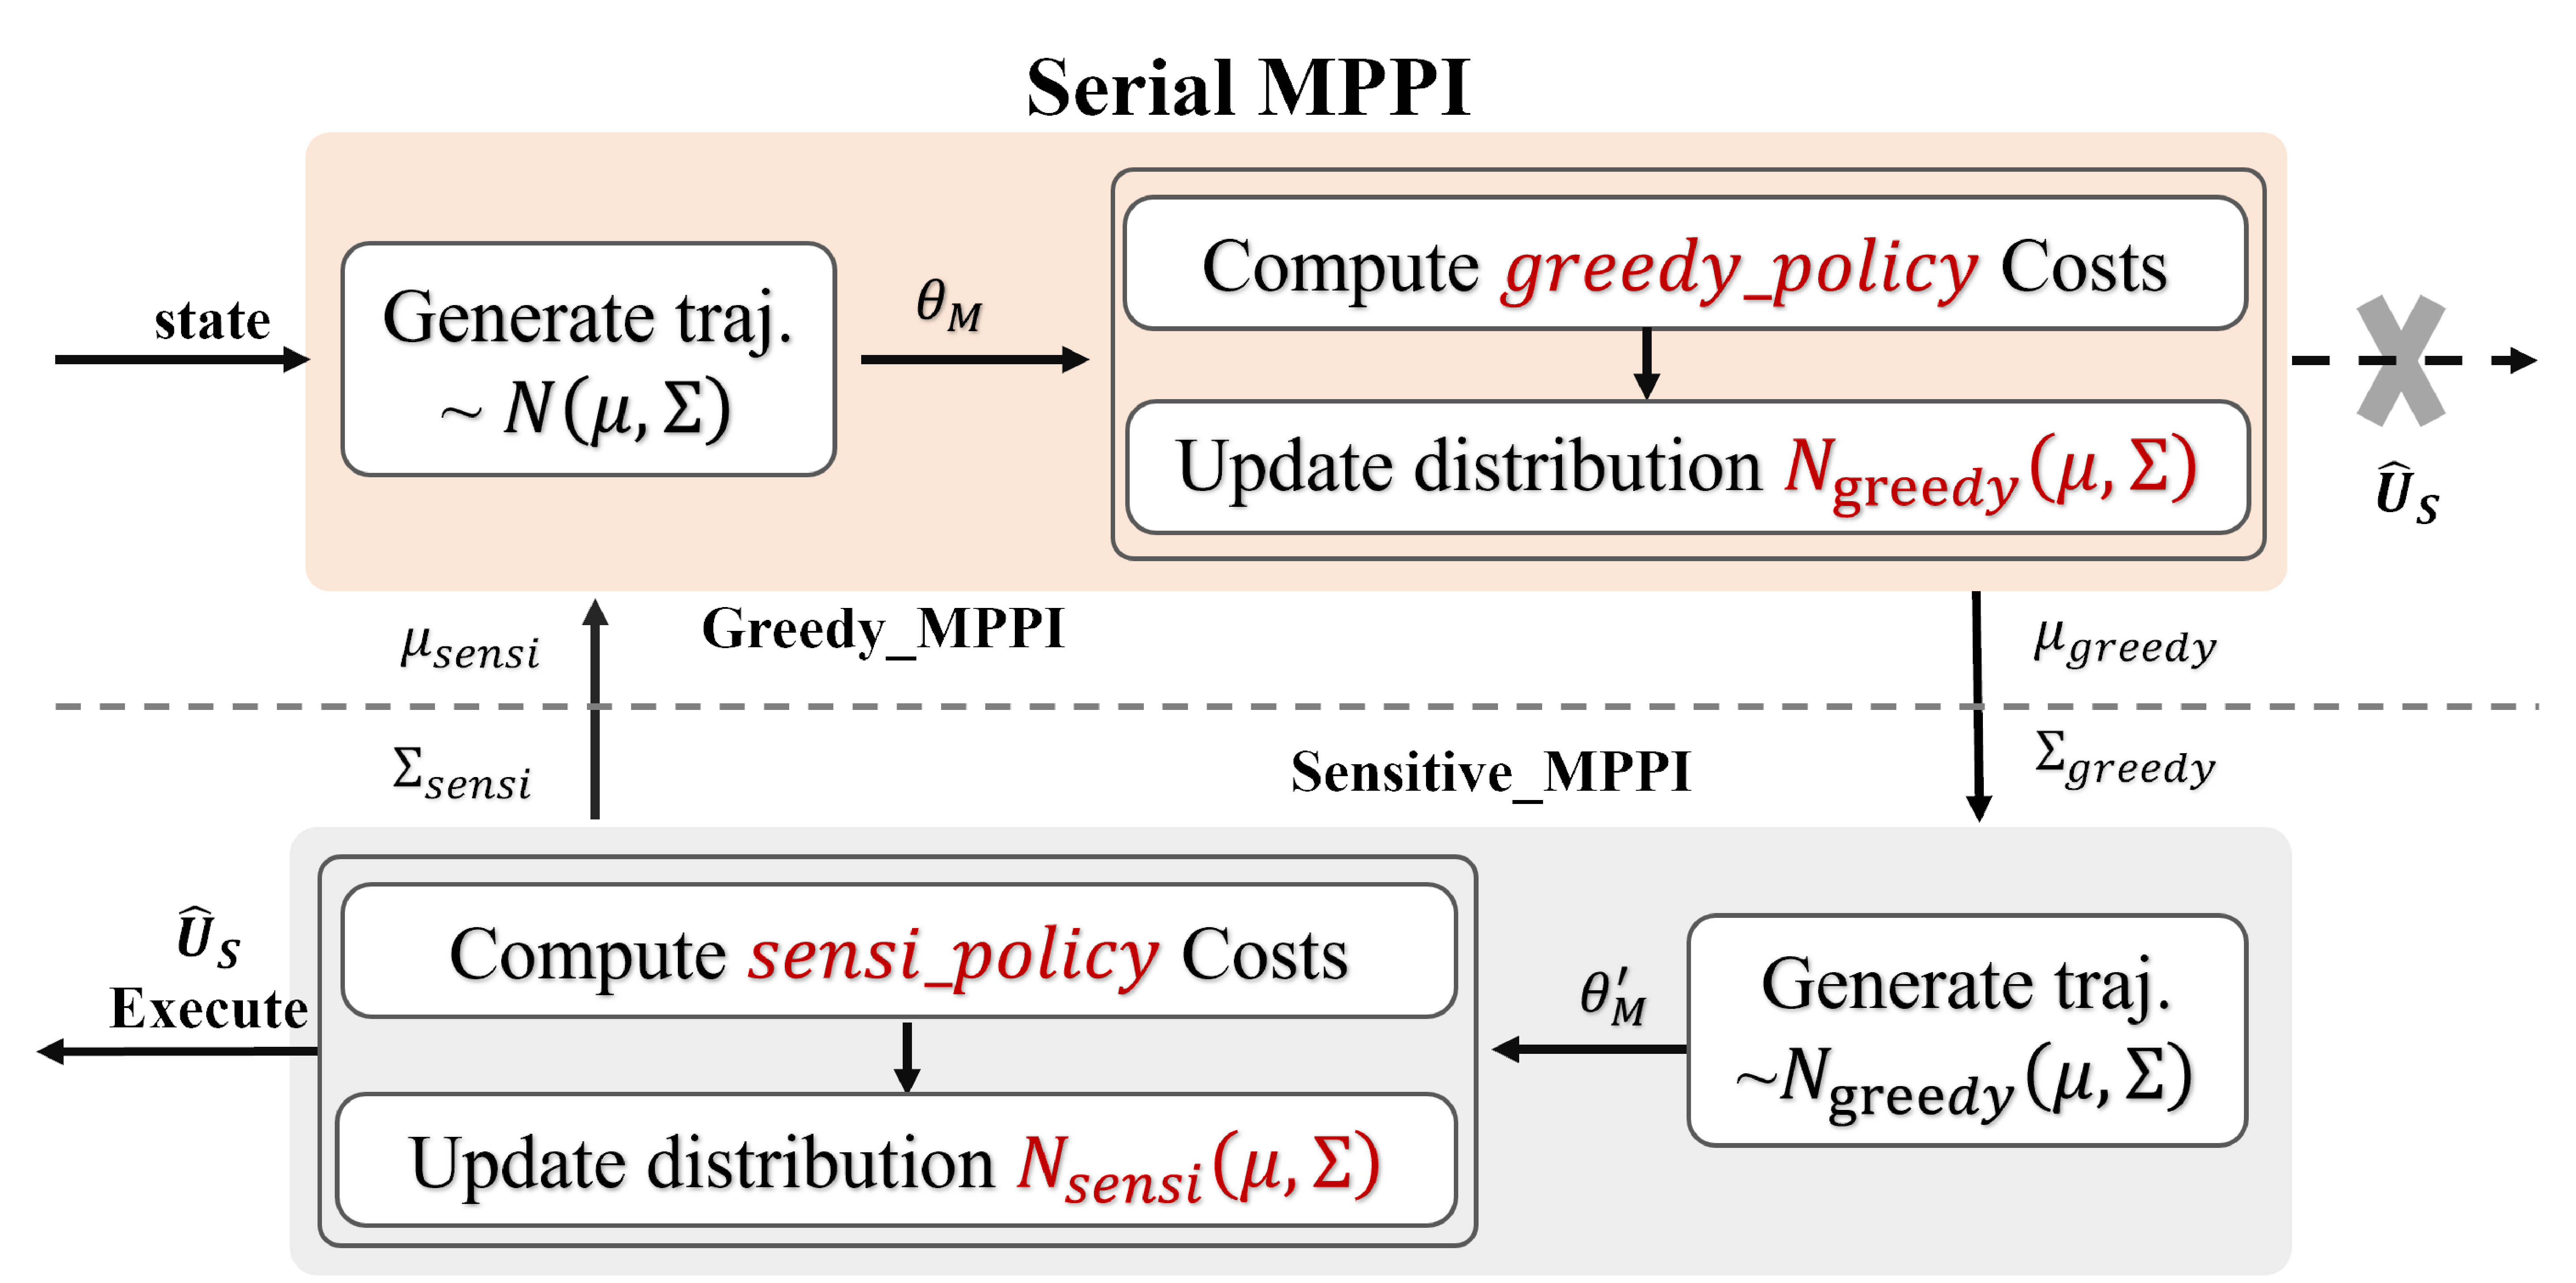
\includegraphics[width=8.5cm]{serialMPPI.eps}
	\caption{The control sequences \(\hat{U}_{S}\) from Greedy-MPPI are used as the sampling mean  \(\hat{\mu}_{S}\) for Sensitive-MPPI. By substituting the policy with higher sensitivity to the environment, trajectories prone to collisions are optimized to safer regions.}\label{FIG_1}
\end{figure}

In theory, Serial MPPI can enhance exploration capability and improve the safety of the single-layer MPPI planned trajectories. However, this potential comes at an additional computational cost due to the extra steps involving sampling and rolling out the dynamic model at each optimizer iteration.

To overcome this problem, this paper proposes a more efficient algorithm architecture, Parallel MPPI, which streamlines the optimization process by requiring only one sampling operation per iteration. This achieves superior planning performance compared to both single-layer MPPI and Serial MPPI while minimizing computational overhead.

\begin{figure}[h]\centering
	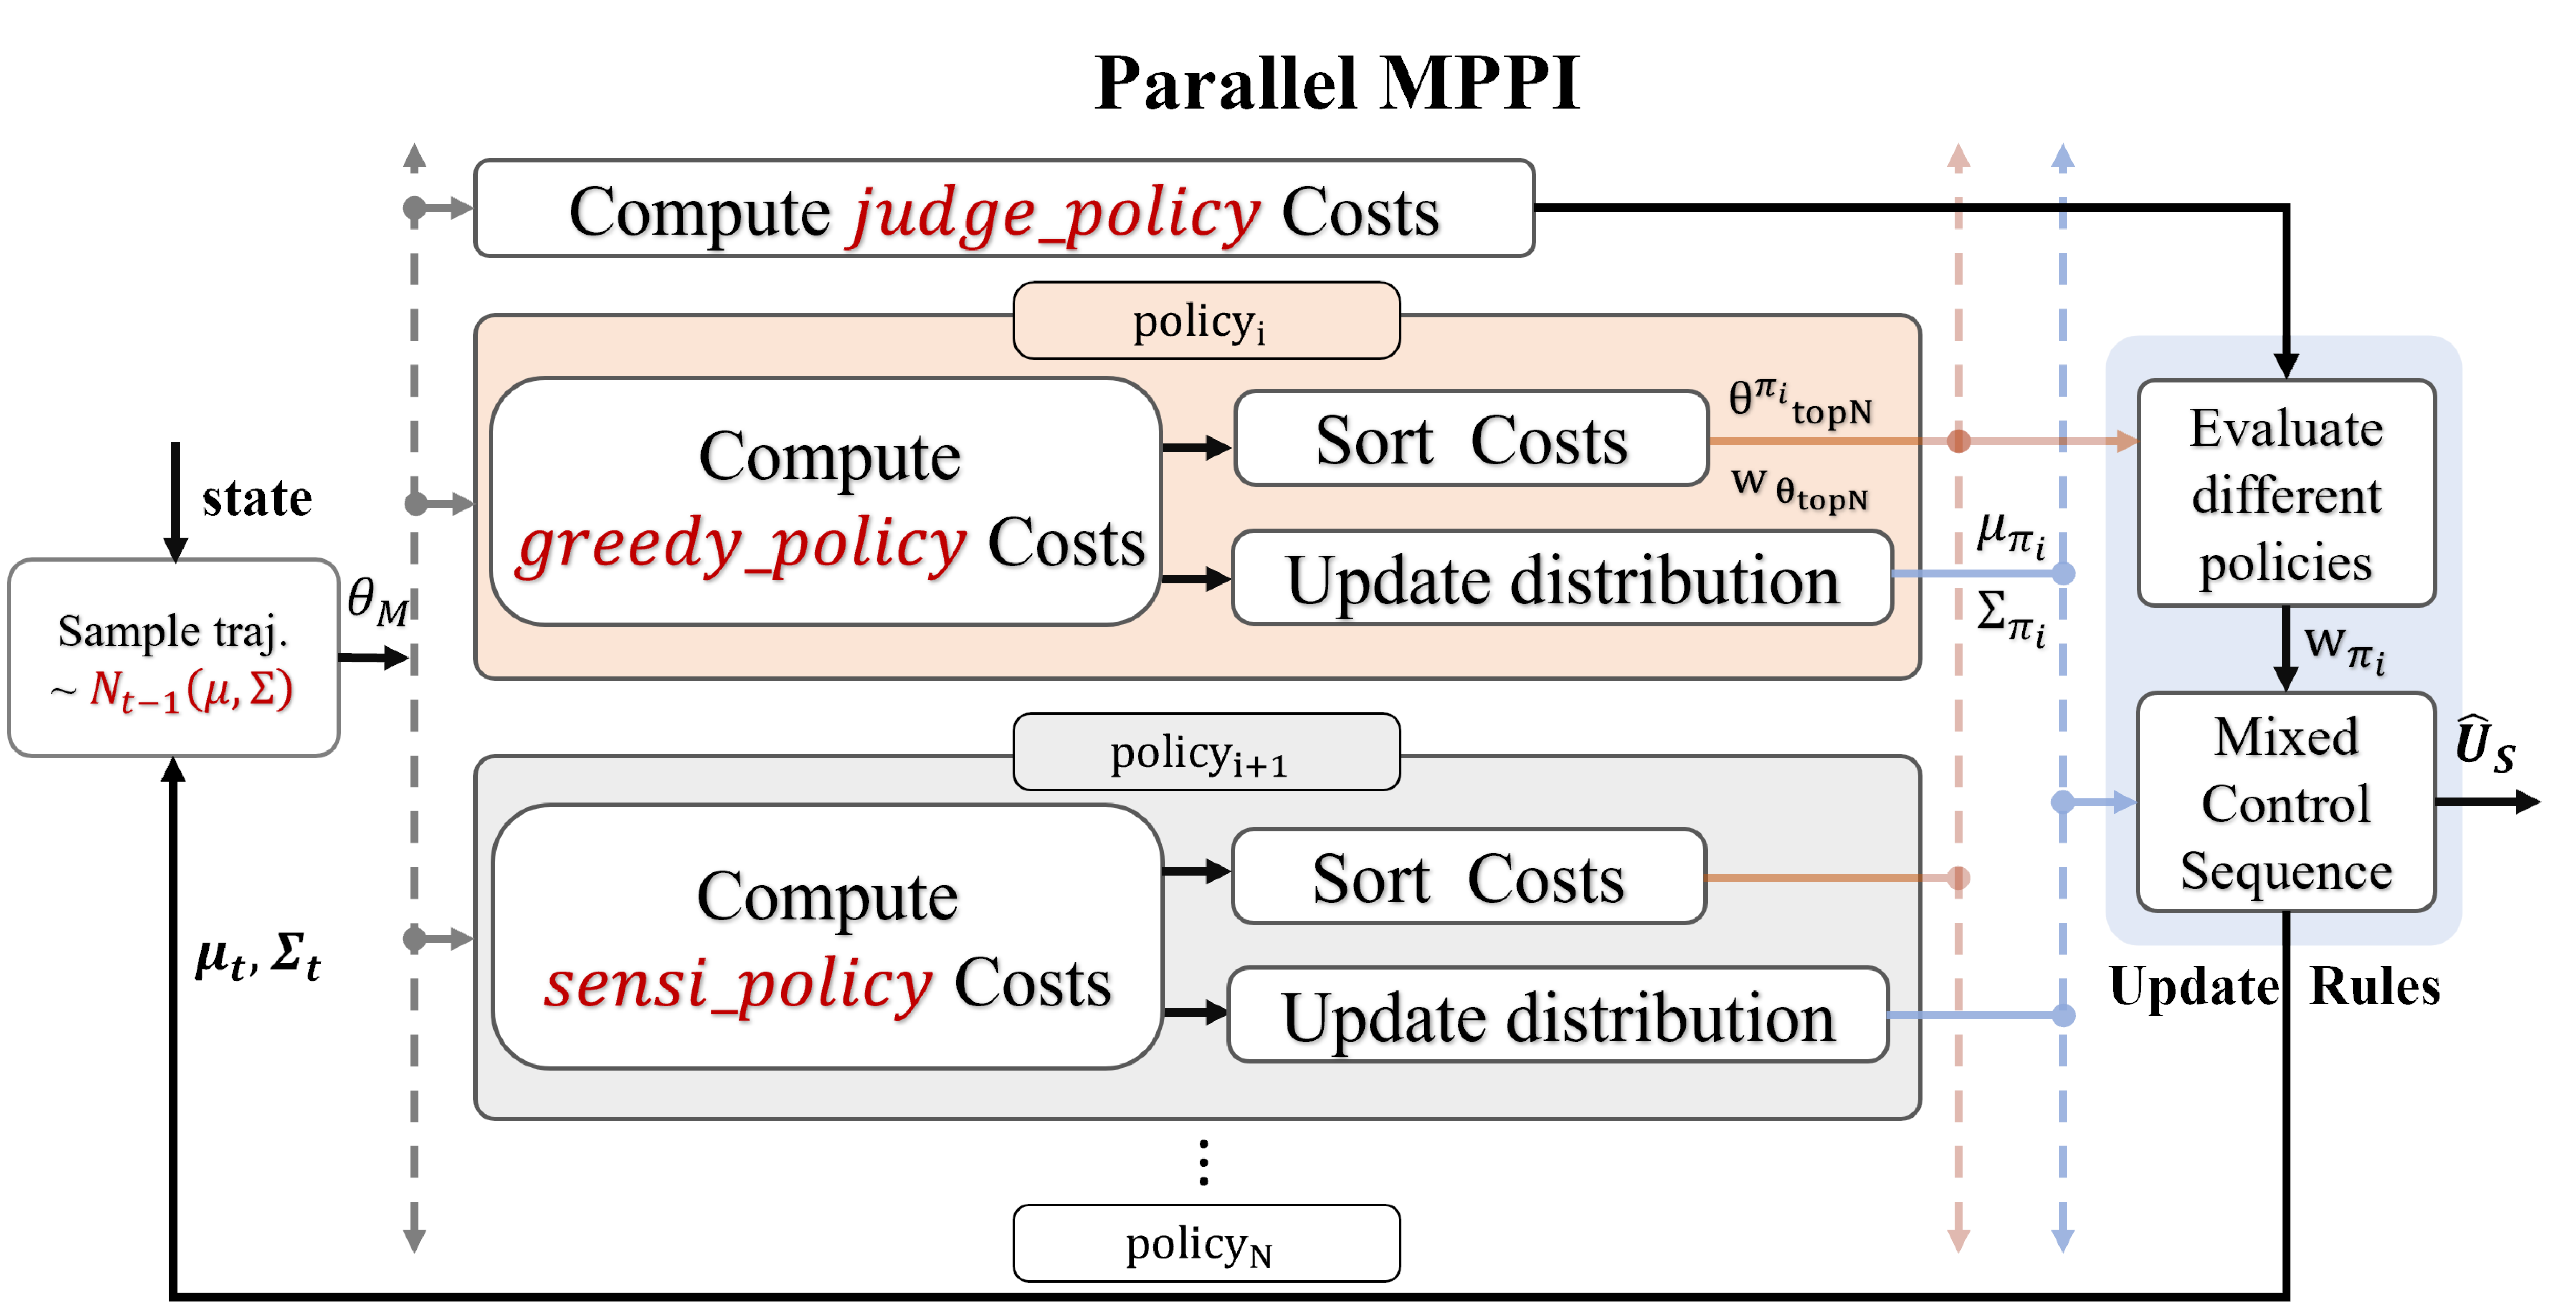
\includegraphics[width=8.5cm]{ParallelMPPI.eps}
	\caption{ Parallel MPPI, which streamlines the optimization process by requiring only one sampling operation per iteration.}\label{FIG_2}
\end{figure}

\subsection{Parallel MPPI Problem Statement}

The main challenge is to develop an effective approach for automatically mixing or selecting one from the multiple control sequences concurrently generated by parallel MPPI planners with different policies, such as one policy focusing on quickly reaching the target position while another leaning towards steering paths away from obstacles, based on the current robot and environment state, and other dynamical constraints, to swiftly and safely accomplish planning tasks, minimizing time costs and reducing collision risks.

\section{Parallel MPPI}

This paper extends concepts from MME-DDP[1] and MPQ[2] to derive the strategy selection method for Parallel MPPI.

MME-DDP[1] introduces a practical method for Multi-modal DDP. It employs softmax functions to assign weights to different planned paths based on their Value function \( {{V}^{(n)}}(t,{{x}_{t}}) \) , which quantifies the quality or performance of paths planned by each DDP with different policies.

MPQ[2] derives the value function of MPPI to quantify its planned trajectories. 

\subsection{Derivation of the Parallel MPPI Formula}


The evaluation of paths planned by each MPPI with different policies is conducted under a unified evaluation standard provided by the Judge Policy. In Parallel MPPI, softmax functions are employed to update weights for multiple planned paths based on its Value function, which is provided by MPQ to quantify the quality of these paths.

The form of combining multiple control sequences resembles the approach of a "Mixed Gaussian Distribution" : 

\begin{align}
	{\mu _{t,h}} & = (1 - {\alpha _\mu }){\mu _{t - 1,h}} + {\alpha _\mu }\sum\nolimits_{i = 1}^{{N_{policy}}} {{w_i}{\pi ^i}(u|x)} \tag{6}\\
    {\Sigma _{t,h}} & = (1 - {\alpha _\sigma }){\mu _{t - 1,h}} + {\alpha _\sigma }\sum\nolimits_{i = 1}^{{N_{policy}}} {{w_i}\Sigma _{t,h}^i}i \tag{7}\\
	{w_i} =& \frac{{\exp ( - \frac{1}{\alpha }({V_{policy(i)}} - {V_{policy(i)}}.\min ()))}}{{\sum\nolimits_{i = 1}^{{N_{policy}}} {\exp ( - \frac{1}{\alpha }({V_{policy(i)}} - {V_{policy(i)}}.\min ()))} }} \tag{8} 
\end{align}

Inspired by MPQ, the Value function of MPPI can be formulated as follows:
\begin{align}
	\nonumber	{V_{\text{policy}(i)}} = -\lambda \log E\bigg[ \exp \bigg( -\frac{1}{\lambda} \Big( & \sum_{l=1}^{H-1} {c_{\pi^*}}({s_{t + l}},{a_{t + l}}) \\
	 + {Q^{\pi^*}}({s_{t + H}},&{a_{t + H}}) \Big) \bigg) \bigg]
	\tag{9}
\end{align}
We assume that $\sum\nolimits_{l = 1}^{H - 1} {{c_{\pi^*}}} \left( {{s_{t + l}},{a_{t + l}}} \right)$ denotes the cost function of $TopN$ trajectories sampled from policy 
${\pi _i}$ but evaluated on the judge policy \(\pi^*\). Ignore ${Q^{\pi^*}}\left( {{s_{t + H}},{a_{t + H}}} \right)$ and let
$\mathrm{Cost^{\pi^*}}(i): = \sum\nolimits_{l = 1}^H c \left( {{s_{t + l}},{a_{t + l}}} \right)$ for simplicity.
\begin{align}
\nonumber {V_{policy(i)}} &=  - \lambda \log E\left[ {\exp \left( { -\frac{1}{\lambda}\left( {\sum\nolimits_{l = 1}^H {{c_{\pi^*}}\left( {{s_{t + l}},{a_{t + l}}} \right)} } \right)} \right)} \right] \\
=& - \lambda\log \left( \frac{1}{N }\sum\nolimits_{l = 1}^N {\exp } \left( -
	\frac{1}{\lambda}{\mathrm{Cost}^{\pi^*}}(i) \right) \right) \tag{10}
\end{align}

\noindent {\textbf{Remark.}} \textit{It's important to note that the Judge Policy, distinct from the Greedy/Sensitive Policy, aims to establish a unified evaluation standard and does not participate in generating planning trajectories, solely evaluating the trajectories based on their distance to the target and risk of collisions with the environment.} \\ 
 We refer the readers to Appendix A in [page xx] for more details.

Experimentation revealed that when calculating expectation of $TopN$ trajectories' cost, assigning \textit{normal weight} $\frac{1}{N}$ to each trajectory does not effectively capture the differences between polices. Particularly, when the distribution regions of the $TopN$ trajectories generated by different policies overlap significantly, using  \textit{normal weight} leads to same quantified results.



Using policy-oriented \textit{softmax weight}:
$
\frac{\exp\left(-\frac{1}{\beta}\text{Cost}^{\pi_i}(i)\right)}
{\sum_{l=1}^N \exp\left(-\frac{1}{\beta}\text{Cost}^{\pi_i}(i)\right)}
$
rather than uniform weights $\frac{1}{N}$ allows for a better quantification of differences between policies $\pi^i$.
 Consequently, when submitting trajectories to the Judge Policy, each policy provides not only the planned $TopN$ trajectories but also the corresponding \textit{confidence weights} :
\begin{align}
	\nonumber {V_{\text{policy}(i)}} &= -\lambda \log \left( \sum_{l=1}^N \frac{\exp\left(-\frac{1}{\beta}\text{cost}^{\pi_i}(i)\right)}{\sum_{l=1}^N \exp\left(-\frac{1}{\beta}\text{cost}^{\pi_i}(i)\right)} \cdot \right. \\
	&\qquad  \qquad \qquad \left. \exp\left(-\frac{1}{\lambda}\text{cost}^{\pi *}(i)\right) \right) \tag{11}
\end{align}
 And to avoid potential numerical overflow, let 
\begin{align}
{A_l} &=  - {1 \mathord{\left/
		{\vphantom {1 \beta }} \right.
		\kern-\nulldelimiterspace} \beta }\text{cost}\left( {t^{{\pi _i}}}(i) \right) - {1 \mathord{\left/
		{\vphantom {1 \lambda }} \right.
		\kern-\nulldelimiterspace} \lambda }\text{cost}\left( {t^{\pi *}}(i) \right) \tag{12}\\
{B_l} &=  - {1 \mathord{\left/
		{\vphantom {1 \beta }} \right.
		\kern-\nulldelimiterspace} \beta }\text{cost}\left( {t^{{\pi _i}}}(i) \right) \tag{13}
\end{align}
the final result is: 
\begin{align}
	\nonumber  &{V_{\text{policy}(i)}} = -\lambda \left( \log \sum\nolimits_{l = 1}^N \exp \left( {A_l - A_{\max}} \right) + \right.\\
	&\quad \quad \left. \log \sum\nolimits_{l = 1}^N \exp \left( {B_l - B_{\max}} \right) - A_{\max} + B_{\max} \right) \tag{14}
\end{align}




\subsection{the influence of $\alpha$,$\lambda$,$\beta$}
$\alpha, \lambda,$ and $\beta$ are all used in the policy evaluation step of the Parallel MPPI 
algorithm, but they serve different purposes. The $\beta$ parameter is used to calculate the weights of the $TopN$ trajectories given to the Judge Policy by different policies. It can more fully extract the intrinsic differences between different policies. On the other hand, the $\alpha$ and $\lambda$ parameters only affect the formula for calculating the expected value and do not affect the calculation of the weight function, so they cannot control the differences in weights between different policies.

Using the softmax function with the parameter $\beta$ replaces the original use of uniform weights $1/N$. Here, the role of $\beta$ is:
\begin{enumerate}
	\item By changing the value of $\beta$, you can control the "softness" of the softmax function.
	\item The larger the $\beta$ value, the more uniform the softmax distribution becomes. Differences between function values are less pronounced, and it tends to favor $1/N$.
	\item The smaller the $\beta$ value, the narrower the softmax distribution becomes. Differences between function values are more pronounced, but policy evaluation becomes more extreme.
\end{enumerate}

When $\beta$ is adjusted to an appropriate value, it can better capture the differences between policies. Therefore, the $\beta$ parameter can finely control the weight distribution formed by the softmax function, providing a tunable hyperparameter that makes policy-oriented weights more closely resemble actual policy differences.

\subsection{why Judge Policy}
The Judge Policy provides an independent and objective evaluation standard, enabling the quantification (scoring) and comparison (assessment) of trajectories planned by various policies under the same criteria. This approach avoids direct comparisons using internal standards of each policy. Regardless of the differences in internal standards among policies, they are assessed within a consistent, neutral framework. The core purpose of designing the Judge Policy is to ensure fairness in the evaluation and comparison of different policies, without being influenced by individual policy-specific standards.

\subsection{Parallel MPPI algorithms}


\begin{figure*}[h]\centering
	\includegraphics[width=\textwidth]{ParrallelMPPIiteration3.eps}
	\caption{ Precomputed maps. Taking a 2D image as an example, the SDF Map is obtained by applying EDT on the Voxel/Bool Map, followed by computing the SDF Potential Map for nuanced distance control. The Gradient Map is derived through finite differencing based on the SDF Map}
\end{figure*}



\begin{algorithm}
	\caption{Parallel MPPI}
	\begin{algorithmic}[1]
		\Statex \textbf{Given}: Parallel MPPI Parameters $topN$, $\beta$, $\lambda$, $\alpha$
		
		\While{task not complete}
		\State Sample $M$ trajs. $\theta_{M,t}$ of len. $H$ from $\mathcal{N}(\mu, \widehat{\Sigma}_{t-1})$, $\mu \in \{\widehat{\mu}_{t-1}, \widehat{\mu}_{\pi_i,t-1}\}$
		\Statex \textcolor{lightpurple}{// Evaluate different policies (e.g., Greedy/ Sensitive)}
		\For{each $\pi_i$}
		\For{$k = 1$ to $M$ in parallel}
		\State $Cost^{\pi_i}(\theta_k) := \sum_{l=1}^H c^{\pi_i}(\theta_{k,l})$
		\EndFor
		\State $\widehat{\mu}_{\pi_i,t}, \widehat{\Sigma}_{\pi_i,t}:= $ MPPI\_Base\_Function \Comment{(3-5)}
		\Statex \textcolor{lightpurple}{// Select topN trajs. and assign weight for each }
		\State topN\_index $\leftarrow \text{sort}(Cost^{\pi_i}(\theta_M), topN)$ 
		\State $\theta_{topN} := \theta_M(\text{topN\_index})$
		\State $w_{\theta_{topN}} := 
		\frac{\exp\left(-\frac{1}{\beta}\text{Cost}^{\pi_i}(\theta_{topN})\right)}
		{\sum_{l=1}^{topN} \exp\left(-\frac{1}{\beta}\text{Cost}^{\pi_i}(\theta_{topN})\right)}
		$
		\Statex \textcolor{lightpurple}{// MPPI Value Function}
		\State $V_{\pi_i} := E[Cost^{\text{Judge\_Policy}}(\theta_{topN}, w_{\theta_{topN}},\lambda)]$ \Comment{(14)}
		\EndFor
		\Statex \textcolor{lightpurple}{// Update mixed Gaussian weight using $V_{\text{policy}(i)}$}
		\For{each  $\pi_i$}
		\State $w^{\pi_i} := \text{Softmax}(-\frac{1}{\alpha} V_{\pi_i})$
		\EndFor
		\State $\widehat{\mu}_t := (1 - \alpha_\mu)\widehat{\Sigma}_{t-1} + \alpha_\mu\sum_{i=1}^{N_{\text{policy}}} w^{\pi_i}\widehat{\mu}_{\pi_i,t}$
		\State $\widehat{\Sigma}_t := (1 - \alpha_\sigma)\widehat{\Sigma}_{t-1} + \alpha_\sigma\sum_{i=1}^{N_{\text{policy}}} w^{\pi_i}\widehat{\Sigma}_{\pi_i,t}$
		
		\EndWhile
	\end{algorithmic}
\end{algorithm}

In this section, we introduce the Parallel MPPI algorithm.
Line 2 samples a batch of control sequences \(\left\{u_{i, h}\right\}_{i=1 . . . M}^{h=1 . . H}\) of size \(M \times H\) from  $\mathcal{N}(\mu, \widehat{\Sigma}_{t-1})$. Roll out the dynamic model to obtain $M$ trajectories $\theta_{M,t}$  of length H.
Lines 3 to 12 evaluate different policies (e.g., Greedy and Sensitive). More specifically,
Lines 4 to 7 run the basic MPPI algorithm, computing the cost function $Cost^{\pi_i}(\theta_M)$ designed by the corresponding policy and  utilizing the softmax to obtain $\widehat{\mu}_{\pi_i,t}, \widehat{\Sigma}_{\pi_i,t}$. 
Lines 8 to 12 determine the evaluation results for each policy. The policy selects the top N trajectories $\theta_{topN}$ with the lowest cost values and assigns confidence weights $w_{\theta_{topN}}$ to each trajectory. These trajectories are then collectively submitted to the Judge Policy, which calculates scores based on the derived evaluation formula (Equation 6).
Lines 13 to  15  compute Policy Weight.
Based on the value function $V_{\pi_i}$ corresponding to each policy, the softmax is used to assign weights for each policy.
Lines 16 to 18 update the mixed mean $\widehat{\mu}_t$ and covariance $\widehat{\Sigma}_t$ based on the policy weights.

This comprehensive process of sampling, evaluating, and updating iterates until the completion of the task, providing an adaptive and efficient approach to trajectory planning in the context of multiple policies.

\textbf{Remark.} \textit{The mean $\mu$ includes $\widehat{\mu}_{\pi_i,t-1}$ generated by the Greedy and Sensitive policies, as well as the $\widehat{\mu}_{t-1}$, which is the combined result of control sequences from different policies. The $M$ trajectories $\theta_{M,t}$ are divided into N trajectories  $\theta_{N,t},\theta_{N\sim 2N,t}$ for each  $\widehat{\mu}_{\pi_i,t-1}$ and $M-2N$ trajectories  $\theta_{M-2N,t}$ for  $\widehat{\mu}_{t-1}$.}

	
\section{Cost Function Design in MPPI}

The cost function plays a pivotal role in the MPPI algorithm. The primary objective of our cost function is to guide the robot, ensuring compliance with dynamic constraints, avoiding collisions with the environment, and rapidly  reaching the target point. Different strategies, such as Greedy and Sensitive policies, express their uniqueness through the tailored design of their respective cost functions. For the dynamic obstacle avoidance task,
the cost function comprises several sub-cost functions, including:
\begin{enumerate}
	\item Dynamic constraint cost function (considering joint acceleration, velocity, position limits, and self-collision constraints).
	\item Goal distance cost function (evaluating distance to the target in joint space and Cartesian space).
	\item Environment collision cost function (calculating costs between key points of the robotic arm and the SDF/Gradient Map).
\end{enumerate}

This paper introduces a series of optimization tricks to enhance the MPPI cost function. 
Inspired by the application of SDF in dynamic 2D navigation, we extend the method to robotic arms by comprehensively considering the robot's current velocity and SDF gradient direction. 
We deviate from conventional approaches that use manipulability indices to optimize the manipulator configuration, opting instead for a multi-processing approach using  Track-IK to calculate the target joint position based on the current joint state. 
Additionally, in order to improve task completion accuracy, we adopt the Sparse Reward method to minimize the end effector pose errors.  

\section{Enhanced SDF for manipulator}
\subsection{The robot body representation}

When using SDF for collision detection of robotic arms, the robot body is often approximated as a set of overlapping spheres. Specifically, the spheres can be simplified as a set of key points $pts^{'}$ on the robotic arm and their corresponding radii $r$.

The spheres are grouped according to  robot links. Given the local coordinate $pts^{'}(\text{link}_i)$ of spheres under $\text{link}_i(i=1,...,L)$ and the joint state $q_t$, the spheres' position in the workspace $pts(\text{link}_i)$ can be obtained through a simple coordinate transformation using the kinematic model:
\[pts(\text{link}_i) = T(\text{base\_to\_link}_{i}) * pts^{'}(\text{link}_i) \tag{15} \]

In this way, environment collision detection for robot arm  is simplified to a three-dimensional collision query problem of sets of spheres: querying whether the SDF value corresponding to any key point $pts$ is less than a threshold $r+\epsilon$.

This paper establishes a mapping between joint velocity $\text{Vel}(q_t)$ and key point velocity $\text{Vel}(pts)$. Assuming MPPI generates $M$ batches of joint trajectories $\left\{q_{i, h}\right\}_{i=1,...,M}^{h=1,...,H}$ of length $H$, the corresponding trajectories of key points in the workspace $\left\{{pts}_{i, h}\right\}_{i=1,...,M}^{h=1,...,H}$ are calculated using Equation 15.

Joint velocity $\text{Vel}(q_{i,h})$ is obtained through simple differentiation. Similarly, the key point velocities $\text{Vel}(pts_{i,h})$ are computed using the following differentiation matrix:

\[
\begin{bmatrix}
	-1 \!&\!  1 \!&\!  0  \!&\!  \cdots \!&\!  0 \!&\!  0 \!&\!  0  \\
	0 \!&\!  -1 \!&\!  1  \!&\!  \cdots \!&\!  0 \!&\!  0 \!&\!  0  \\
	0 \!&\!  0 \!&\!  -1  \!&\!  \cdots \!&\!  0 \!&\!  0 \!&\!  0  \\
	\vdots \!&\!  \vdots \!&\!  \vdots  \!&\!  \ddots \!&\!  \vdots \!&\!  \vdots \!&\!  \vdots \\
	0 \!&\!  0 \!&\!  0  \!&\!  \cdots \!&\!  -1 \!&\!  1 \!&\!  0  \\
	0 \!&\!  0 \!&\!  0  \!&\!  \cdots \!&\!  0 \!&\!  -1 \!&\!  1  \\
	0 \!&\!  0 \!&\!  0  \!&\!  \cdots \!&\!  0 \!&\!  0 \!&\!  -1  \\
\end{bmatrix}\!
\begin{bmatrix}
	\text{Pos}_1  \\
	\text{Pos}_2  \\
	\text{Pos}_3  \\
	\vdots   \\
	\text{Pos}_{H-2}  \\
	\text{Pos}_{H-1}  \\
	\text{Pos}_{H}  \\
\end{bmatrix}
\!=\!
\begin{bmatrix}
	\text{Vel}_1 \\
	\text{Vel}_2  \\
	\text{Vel}_3  \\
	\vdots   \\
	\text{Vel}_{H-2}  \\
	\text{Vel}_{H-1}  \\
	\text{Vel}_H  \\
\end{bmatrix} \tag{16}
\]

Here, $\text{Pos}_1, \text{Pos}_2, \ldots, \text{Pos}_H$ represent key point positions at different time steps, and the matrix relates them to corresponding key point velocities $\text{Vel}_1, \text{Vel}_2, \ldots, \text{Vel}_H$.

\subsection{SDF Map Creation} 
\textbf{W}e begin with a boolean voxel representation of the environment, known as voxel grid, obtained directly from point cloud .
A signed Euclidean Distance Transform (EDT) is then applied to the voxel grid to generate a SDF map, which represents, for each voxel point $x$, the minimum distance $d(x)$ to the nearest obstacle boundary, The distance values are negative for points inside obstacles, zero at obstacle boundaries, and positive outside of obstacles.

Inspired by the application of the inflation layer in car navigation, we adapt a similar concept to robotic arms. Building upon the SDF Map $d(x)$, we design a corresponding workspace potential function, also referred to as the SDF-Potential map  $\Phi(x)$. This allows for a finer control of the distance between the robot and obstacles, providing increased safety margins in proximity to obstacles.
\[
\Phi(x)=\left\{ 
\begin{array}{c}
	1  \\
	\exp (-\beta (d(x)-\sigma ))  \\
	0  \\
\end{array}
\begin{array}{l}
	,  \\
	,  \\
	,  \\
\end{array}
\begin{array}{l}
	\text{if } d(x) < \sigma \\
	\text{if } \sigma \le d(x) \le \tau  \\
	\text{otherwise}
\end{array}  \tag{17} 
\right. 
\]
where $ \text{inscribed radius } \sigma = r+\epsilon$ , inflation radius is $ \tau $.

The SDF-Gradient map $\text{Grad}(x)$ indicates the direction of steepest change at each point $x$ in the SDF map $d(x)$. We compute the gradient in the $i \in {x,y,z}$ directions using central finite differencing:
\[\text{Grad}(x) = \frac{{\partial d}}{{\partial {x_i}}}(x) \approx \frac{{d(x + \delta {{\bf{e}}_i}) - d(x - \delta {{\bf{e}}_i})}}{{2\delta }}\tag{18} \]
where  $\bf{e}_i$ is the corresponding basis vector.





\subsection{GVOM SDF Cost}

\begin{figure}[t]\centering 
	\includegraphics[width=8.5cm]{collisioncost_c.eps} 
	\caption{GVOM-SDF Cost.}
\end{figure}


Previous works that incorporated SDF into the MPPI cost function exhibited issues where the robot could rapidly pass through $\text{Coll}_{p}(x)$ or get stuck close to obstacles $\text{Coll}_{pv}(x)$.

To address this, our method $\text{Coll}_{ppv\theta}(x)$ introduces dynamic modulation of the SDF cost based on the robot's current velocity and the SDF gradient.
Let the gradient represent the direction of steepest descent in SDF map.
If the robot's velocity and gradient directions are aligned, indicating the robot is moving away from obstacles, the cost is lowered to encourage that motion and avoid stopping near obstacles.
Whereas if the velocity and gradient directions are misaligned, indicating movement towards obstacles, the cost is increased to discourage that behavior and avoid rapid passing through obstacles just to minimize accumulated cost.

In the case of a 2D mass point, $x_{\text{link}_i}$ is the position of the robot; for N-DOF robot arm, $x_{\text{link}_i}$ indicates the point with the minimum SDF value among the key points for each $\text{link}_i$:
\begin{align}
	\text{Coll}_{p} &= \sum\nolimits_{i=1}^{N} {\Phi(x_{\text{link}_i})} \tag{19}\\
	\text{Coll}_{pv}&= \sum\nolimits_{i=1}^{N} {\Phi(x_{\text{link}_i})} \cdot \left\| \text{Vel}(x_{\text{link}_i})\right\|   
	\tag{20} \\
	\nonumber \text{Coll}_{ppv\theta} &= \sum\nolimits_{i=1}^{N} {\Phi(x_{\text{link}_i})} \\
	 &\phantom{=} + \Phi(x_{\text{link}_i}) \cdot \left\| \text{Vel}(x_{\text{link}_i}) \right\| \cdot (1 - \alpha \cdot \cos(\theta))  \tag{21}
\end{align}
where
\begin{align*}
	x_{\text{link}_i} &= \text{argmin}_{x \in \text{key points}(\text{link}_i)} d(x) \\ 
	\theta &= \cos^{-1}(\text{Grad}(x_{\text{link}_i}), \text{Vel}(x_{\text{link}_i})) \\
	\alpha &\in [0,1]
\end{align*}



\subsection{GVOM-SDF Cost Algorithm }

This section introduces the GVOM SDF Cost algorithm.

Lines 1-3 involve the precomputation of Maps. 
EDT on the Voxel Grid yields the SDF Map, followed by computing the SDF Potential Map for nuanced distance control. The Gradient Map is derived through finite differencing based on the SDF Map.

Lines 4-7 compute environment collision cost.
Line 4 involves updating key point positions using the forward kinematic model. After transformation to the world frame, velocities are obtained via finite differencing. Line 5 identifies the key point with the minimum SDF value for each link from the SDF Map. Line 6 retrieves the values of  SDF Potential and Gradient Maps for the selected points in each link. Line 7 computes the collision cost \(\text{Coll}_{ppv\theta}\).

\begin{algorithm}
	\caption{GVOM-SDF Cost}
	\begin{algorithmic}[1]
		\Statex \textbf{Input:}
		\Statex \quad Voxel Grid obtained from point cloud
		\Statex \quad Robot's key points for each link $pts(link_i)$
		\Statex \quad Current Robot Joint State $q_t$
		\Statex \textbf{Precompute Maps}
		\State \quad SDF Map  $ d(x) \leftarrow EDT(\text{Voxel Grid})$
		\State \quad SDF Potential Map $\Phi(x) \leftarrow \exp(-\beta(d(x) - r)) $ 
		\State \quad SDF Gradient Map $Grad(x) \leftarrow FD(d(x))$ 
		
		\Statex \textbf{Environment Collision Cost}
		\State \quad $pts \leftarrow FK(q_t) , \text{Vel}(pts) \leftarrow FD(pts)$
		\State \quad $pt,  \text{Vel}(pt) \leftarrow \text{argmin}(d(pts(link_i))) $
		\State \quad $\Phi(pt) , Grad(pt) \leftarrow $ Check SDF Maps$(pt)$ 
		\State \quad Compute  cost using Equation 21
	\end{algorithmic}
\end{algorithm}

	
\section{Using Track-IK for Guiding MPC}

We employ multi-processing using Track-IK to guide MPC out of local minima and simultaneously optimize its operability. This method continuously generates IK solutions $q_{\text{des},t}$ based on current joint states $q_t$ and the target Cartesian pose $X_g(p_g,R_g)$, and the corresponding joint-space goal cost $\text{dist}_{joint}$ can also design as :
\begin{align}
	\nonumber q_{\text{des},t} &= \text{Track\_IK}(q_t,X_g)  \\
	\text{dist}_{joint} &= \left\|q_t - q_{\mathrm{des},t}\right\|_{2} \tag{23}
\end{align}


In cases where Track-IK is infeasible or the target pose $X_g(p_g,R_g)$ is outside the robot's workspace, we design a Cartesian-space goal cost $\text{dist}_{cart}$. Given the current robot end-effector pose $X_{ee}(p_{ee},R_{ee})$:
\begin{align}
\nonumber \text{dist}_{cart} =& w_1\left\|\mathbf{p}_{ee}-\mathbf{p}_{g}\right\|_{2} + \\
	& w_2 \cos^{-1}\left(2\left\langle\hat{\mathbf{q}}_{ee}, \hat{\mathbf{q}}_{g}\right\rangle^{2}-1\right) \tag{23}
\end{align}
where $\mathbf{p}_{ee}, \mathbf{p}_{g}$ are the position vectors and $\hat{\mathbf{q}}_{ee}, \hat{\mathbf{q}}_{g}$ are the corresponding quaternions representing the rotation matrices $R_{ee}, R_g$.

\begin{figure}[h]
	\centering
	\begin{subfigure}[b]{0.20\textwidth}
		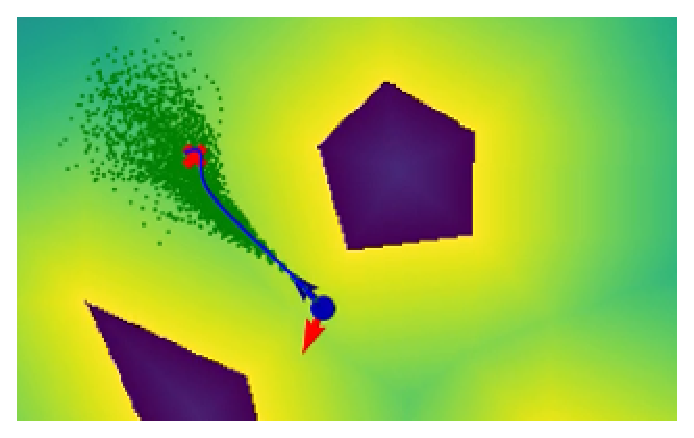
\includegraphics[width=\linewidth]{sparse_reward_No.eps}
		\caption{Without $R\_s(\operatorname{dist})$}
		\label{subfig1}
	\end{subfigure}
	\hspace{-0.2em}
	\begin{subfigure}[b]{0.20\textwidth}
		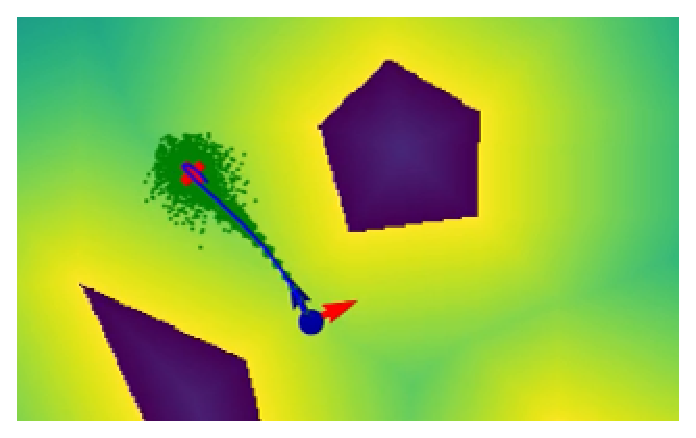
\includegraphics[width=\linewidth]{sparse_reward.eps}
		\caption{With $R\_s(\operatorname{dist})$}
		\label{subfig2}
	\end{subfigure}
	
	\caption{ 
Compare the MPPI-planned paths with and without the sparse reward term for a 2D mass point task aimed at reaching a target while avoiding obstacles. The green points in the plot indicate the sampled trajectories.
The inclusion of $\text{SparseReward}$ results in a rapid cost reduction, prompting sampled trajectories to converge swiftly in the target region, when the distance is within the radius $\sigma$.}
\end{figure}



While the Euclidean norms $\left\|.\right\|_{2}$ in $\text{dist}_{joint}$ and $\text{dist}_{cart}$ drive the robot towards the target pose, they exhibit low sensitivity near the goal, which can result in large errors upon approach.
we integrate it with sparse reward tricks to minimize end-pose error:
\[R\_s(\operatorname{dist})=1-\exp \left(-\operatorname{dist}^{2} /\left(2 \sigma^{2}\right)\right)   \tag{24}\]
Where $\text{dist}$ can be $\text{dist}_{joint}$ or $\text{dist}_{cart}$, and $\sigma$ is the convergence radius.

When dist is within the radius $\sigma$, $\text{SparseReward}$ rapidly decreases costs, driving sampled trajectories to quickly converge in the target region, whereas outside the radius, it has no guiding effect, allowing the robot to automatically slow down near the target location and reduce reach errors.


\section{Results}
\subsection{Robot Dynamic Constraints}

Using the approach from the Paper[STORM], Robot dynamics constraints $C_{safe}$ are designed to protect the safe operation of the robotic arm. This requires considering: Joint Position Bound Limits $C_{joint}$, Joint velocity constraint $C_{stop}$ and self-collision avoidance $C_{self\_coll}$ which uses JointNERF to  accelerate collision query. 
\[C_{safe} = C_{joint} + C_{stop} + C_{self\_coll} \tag{25} \]

\subsection{Differ Policy [Greedy/Sensitive/Judge]}
The  Greedy policy aims to reach the target position quickly with  lower sensitivity to collisions, and assigns a higher weight to the goal-related cost functions:
\begin{align}
\nonumber {C_{greedy}}({x_t},{u_t})= w_g dist+& w_rR\_s(dist)  \\
 	+& w_cColl_{p} + w_sC_{safe} \tag{26}
\end{align}
where $\text{dist}$ can be $\text{dist}_{joint}$ or $\text{dist}_{cart}$. \\
The Sensitive policy is inclined to avoid collisions, exhibiting higher sensitivity to obstacles, and assigning a larger weight to collision-related cost functions:
\begin{align}
	{C_{sensi}}({x_t},{u_t}) =& {w_g}dist + {w_c}Coll_{ppv\theta } +  w_sC_{safe} \tag{27}
\end{align}

the reason  $C_{sensi}$ does not integrate SparseReward is that when the obstacle moves within the target area, the sampled trajectories do not converge in that region, thereby enhancing its exploration capability for obstacle avoidance. This design also indirectly affirms the robust exploratory performance of Parallel MPPI.

The Judge policy focuses solely on the trajectories' distance to the target and their collision status. Thus, the robot dynamics constraints are omitted, and the associated weights are set between those of the Greedy and Sensitive policies:
\begin{align}
	{C_{judge}}({x_t},{u_t}) =& w_gdist + {w_r}R_s(dist) + {w_c}Coll_{ppv\theta } \tag{28}
\end{align}

\textbf{Remark:} There is a misunderstanding that parallel MPPI is meaningless, and the same result can be achieved by continuously tuning the weights of single-layer MPPI.
However, theoretical analysis suggests that the exploration capability of Parallel MPPI  is significantly higher than that of the single-layer MPPI, without sacrificing the convergence of the algorithm. Experimental results and robot motion characteristics indicate that parallel MPPI can adaptively adjust its policy weights based on working conditions: switching to the Sensitive policy to avoid collisions when obstacles are approaching and leaning towards the Greedy policy to accelerate towards the target when obstacles are far away. This motion characteristic, combining the advantages of each strategy, minimizes collisions while striving to complete the task as quickly as possible.


\begin{figure}[h]
	\centering
	\begin{subfigure}[b]{0.11\textwidth}
		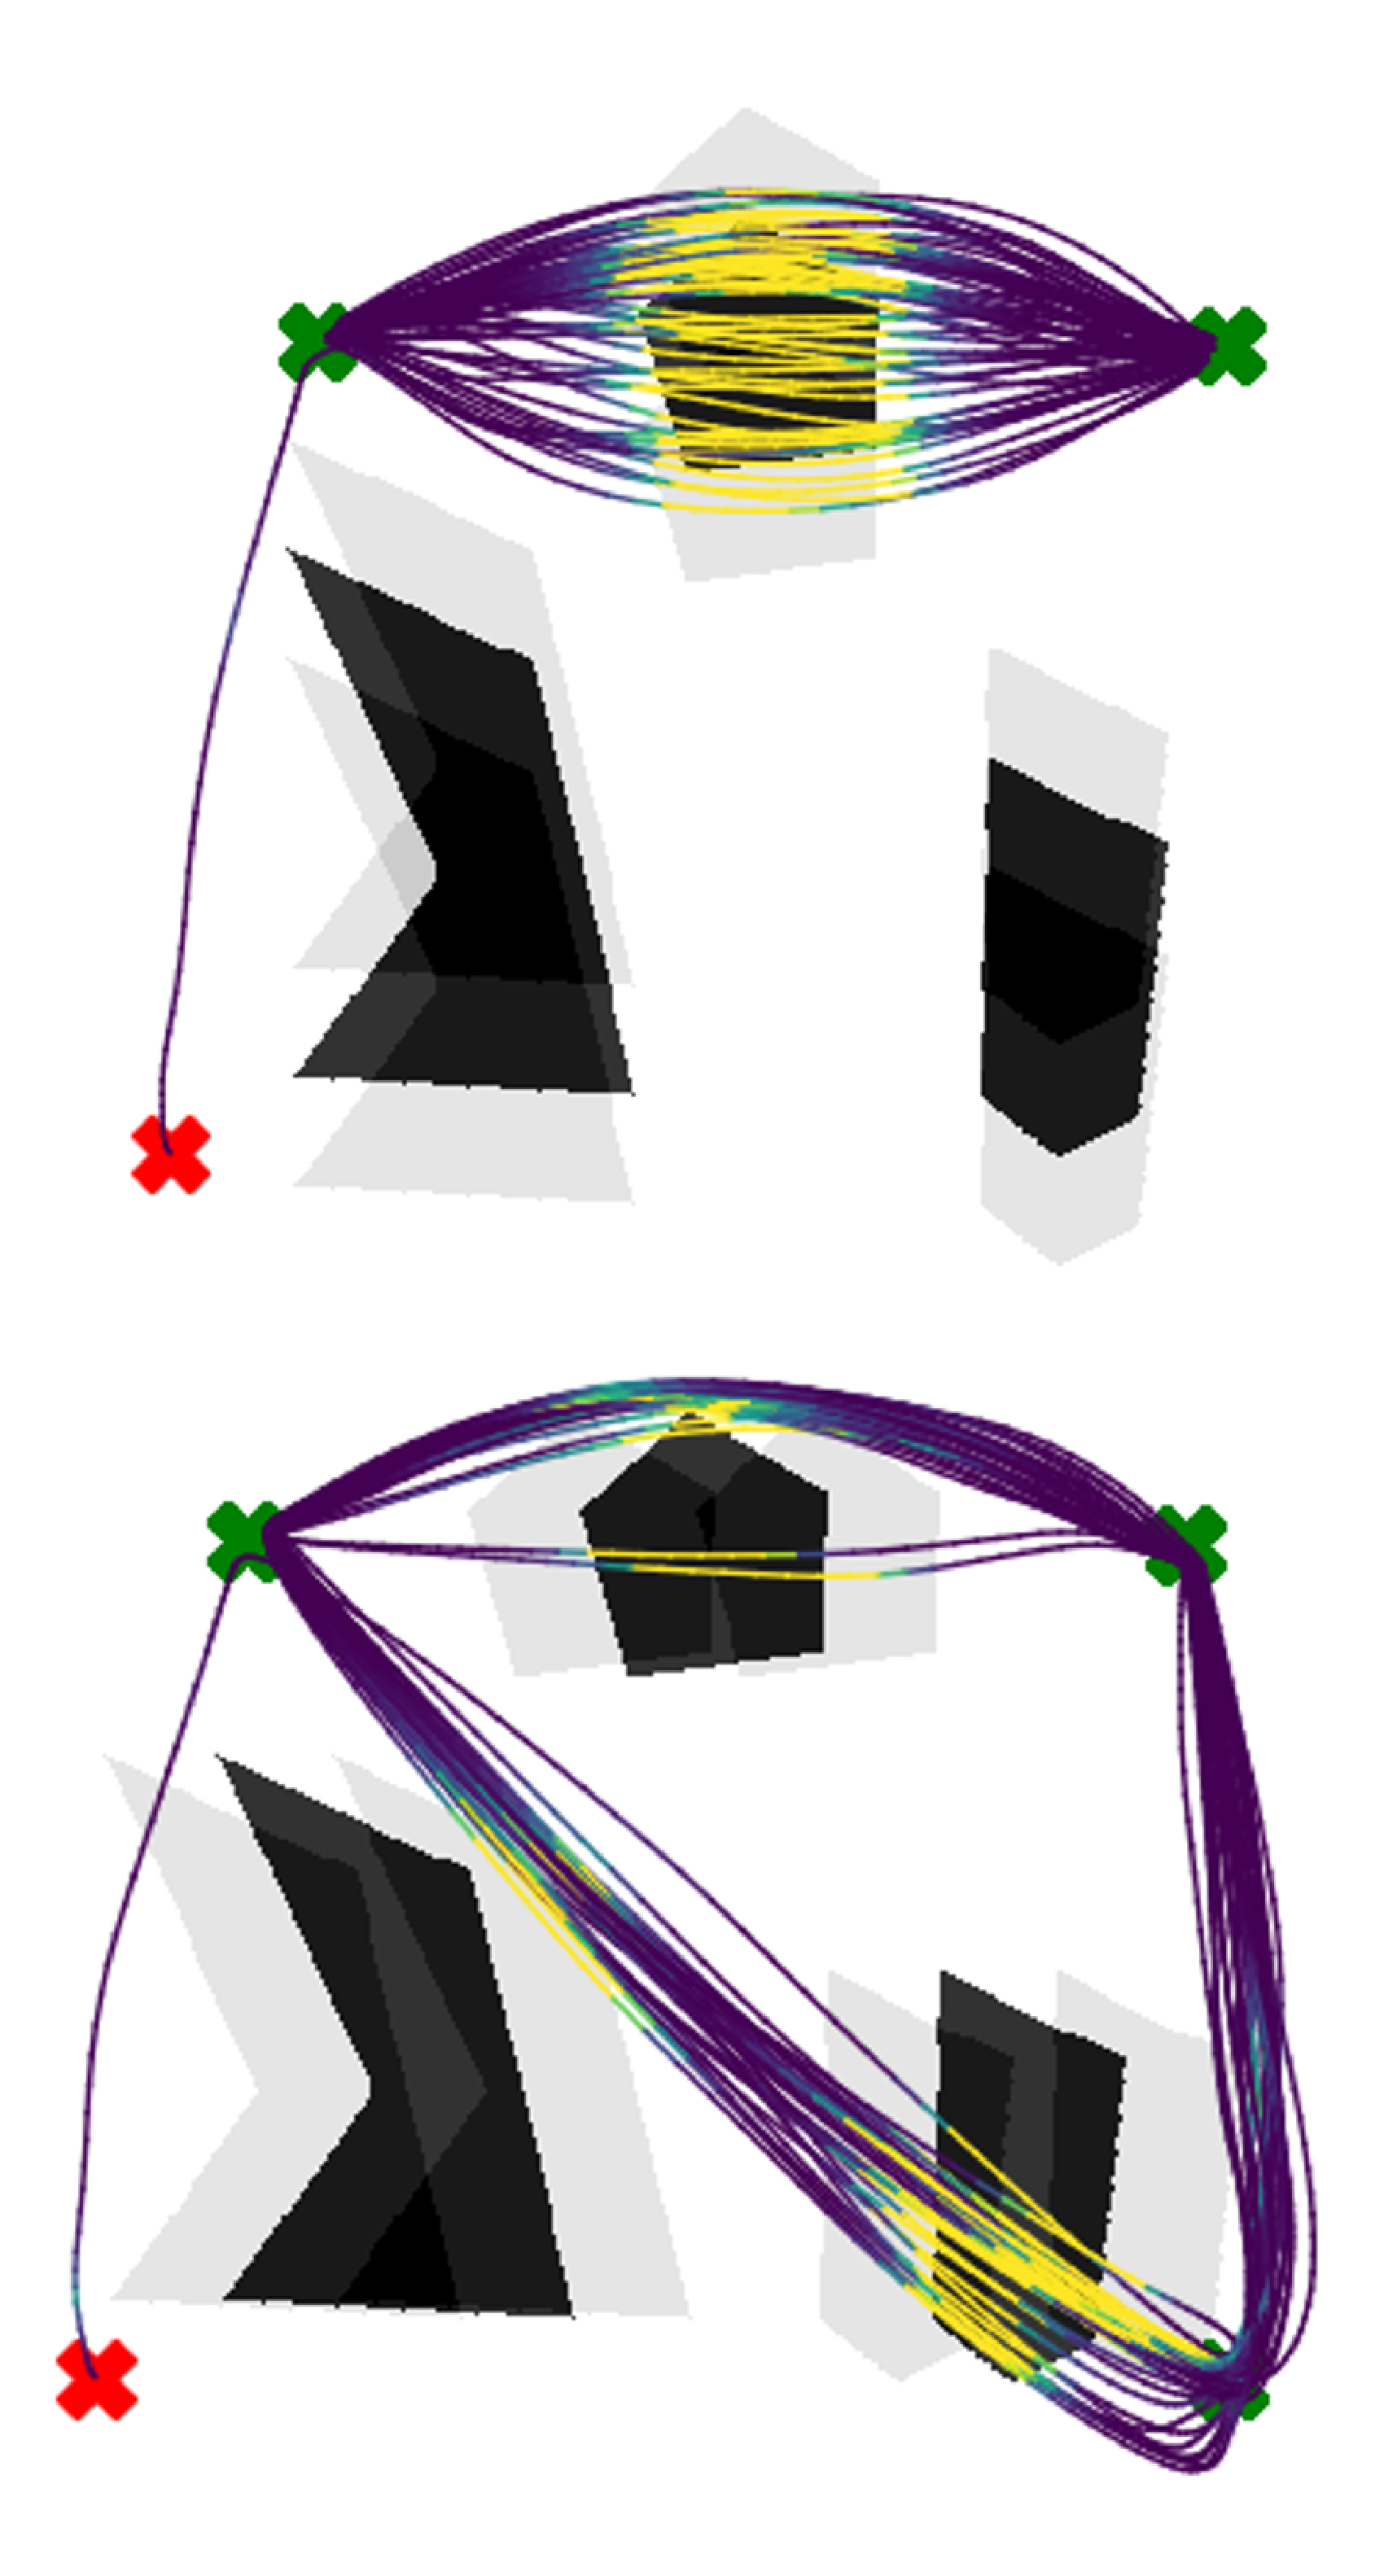
\includegraphics[width=\linewidth]{coll_a.eps}
		\caption{$(a)$}
	\end{subfigure}
	\hfill
	\begin{subfigure}[b]{0.11\textwidth}
		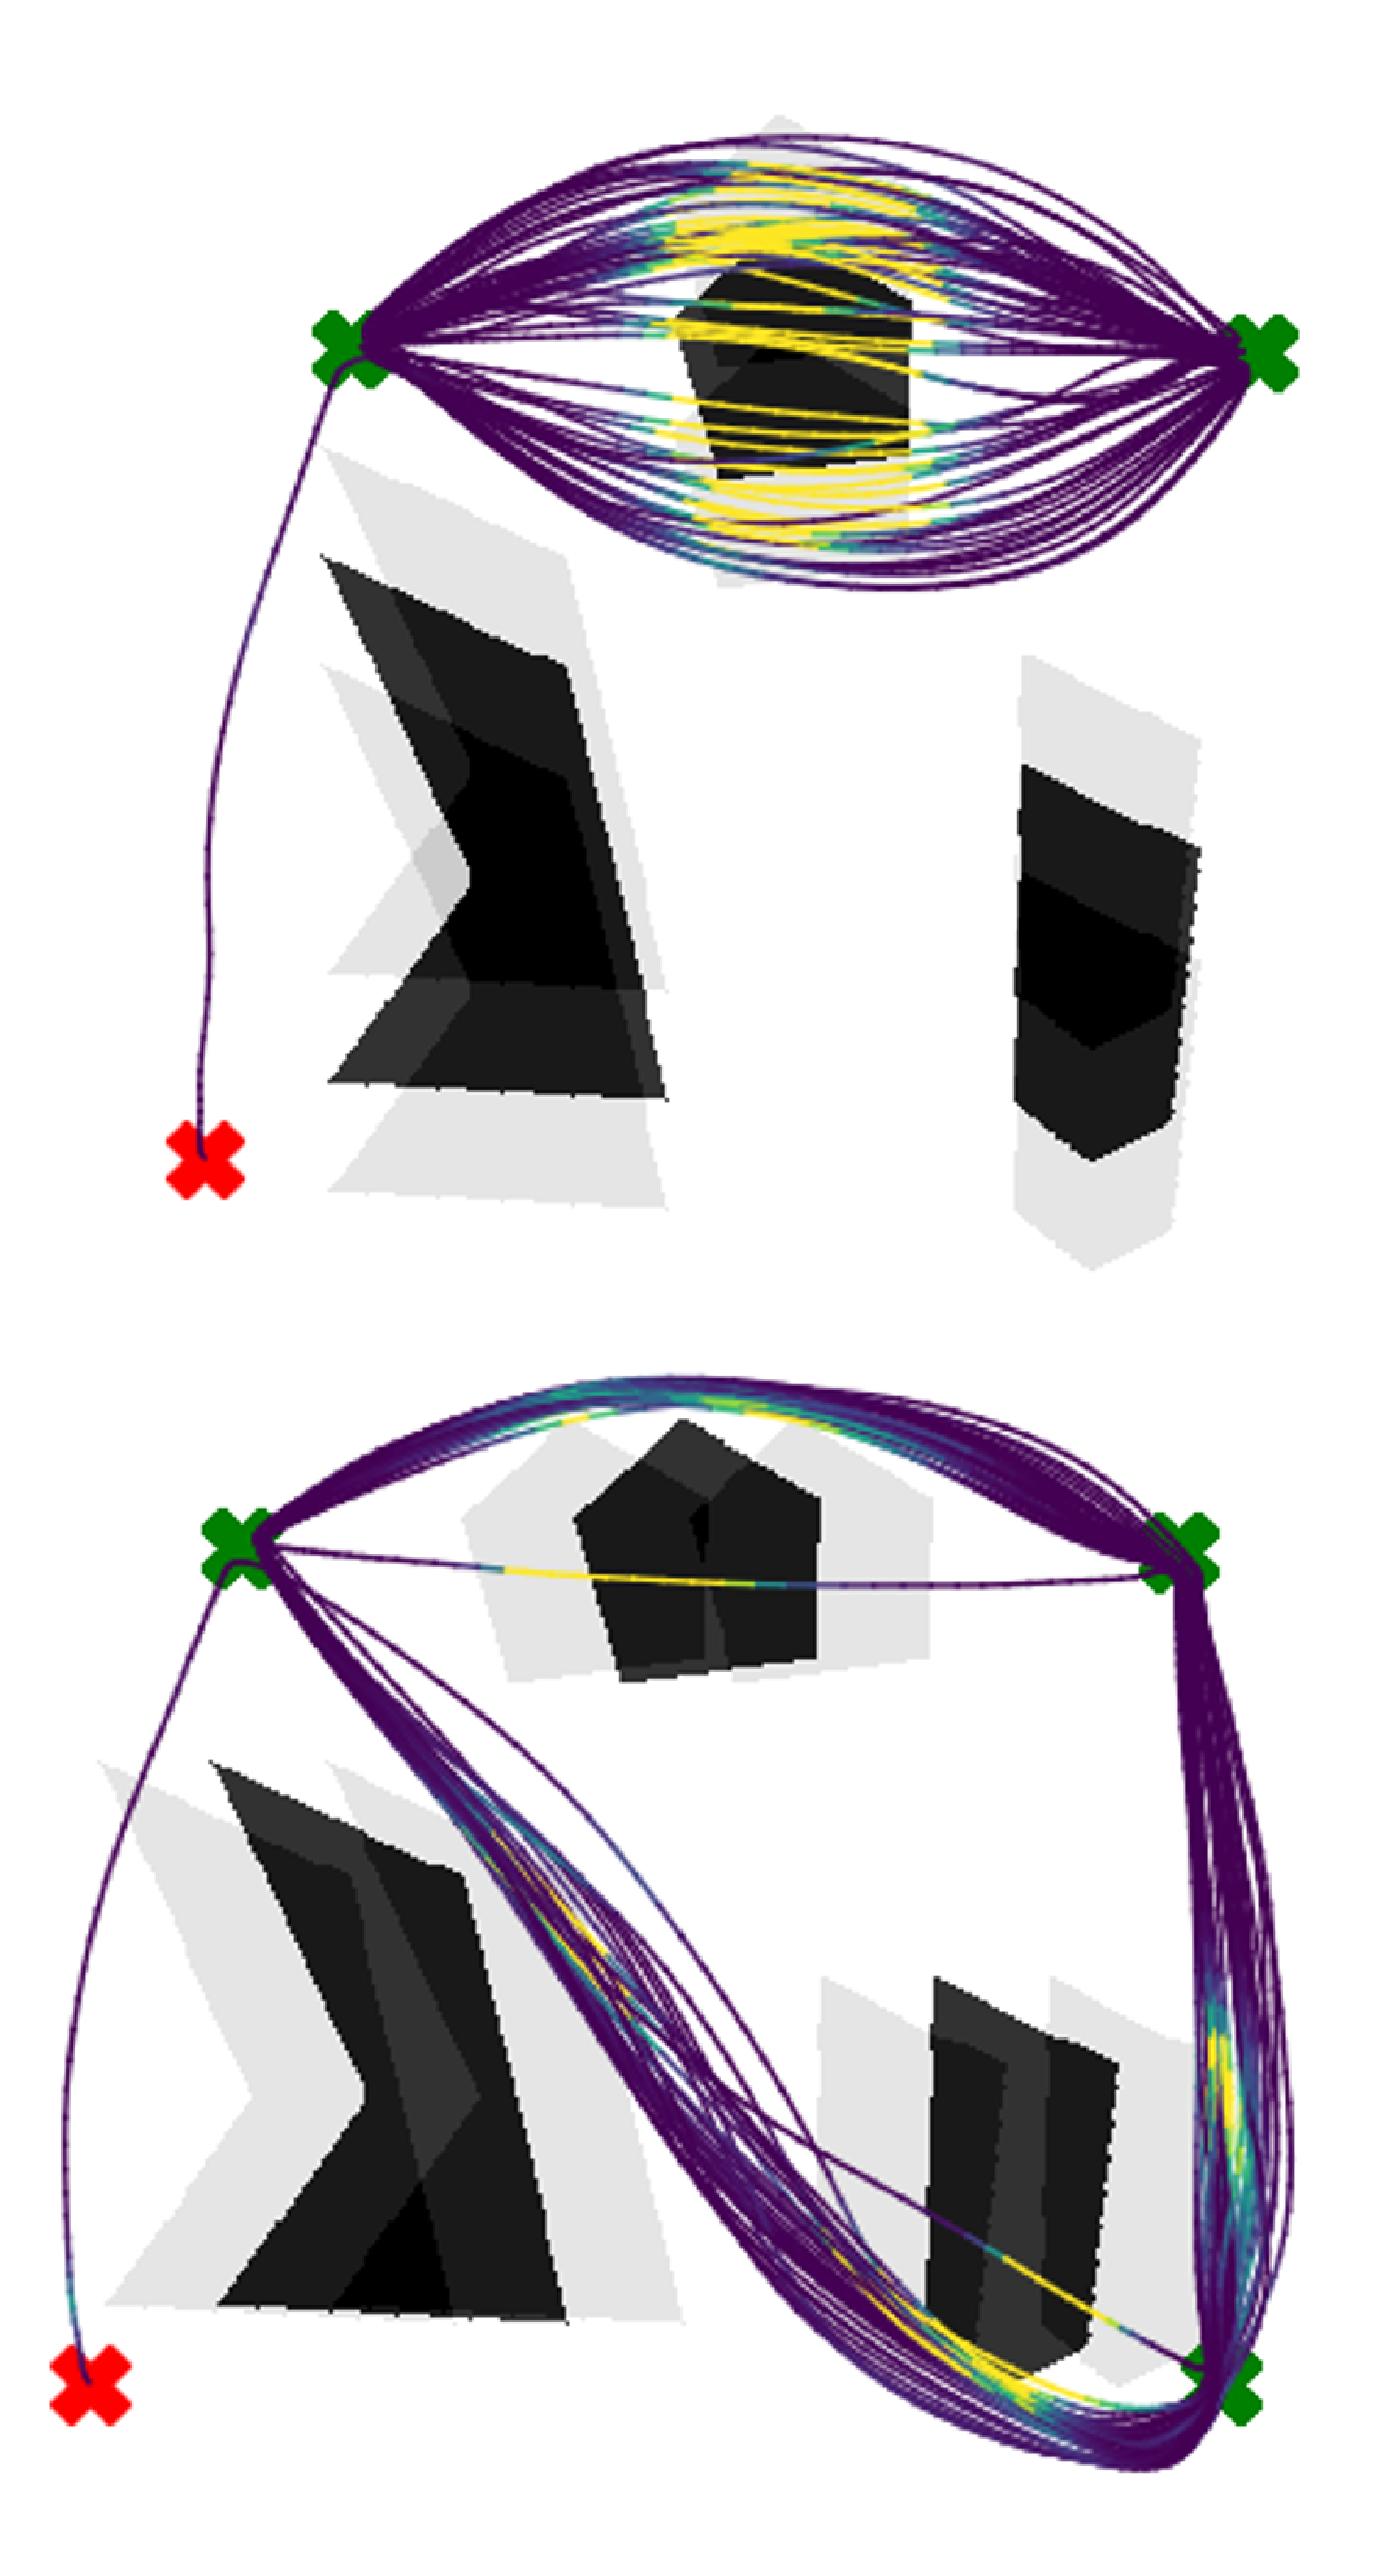
\includegraphics[width=\linewidth]{coll_b.eps}
		\caption{$(b)$}
	\end{subfigure}
	\hfill
	\begin{subfigure}[b]{0.11\textwidth}
		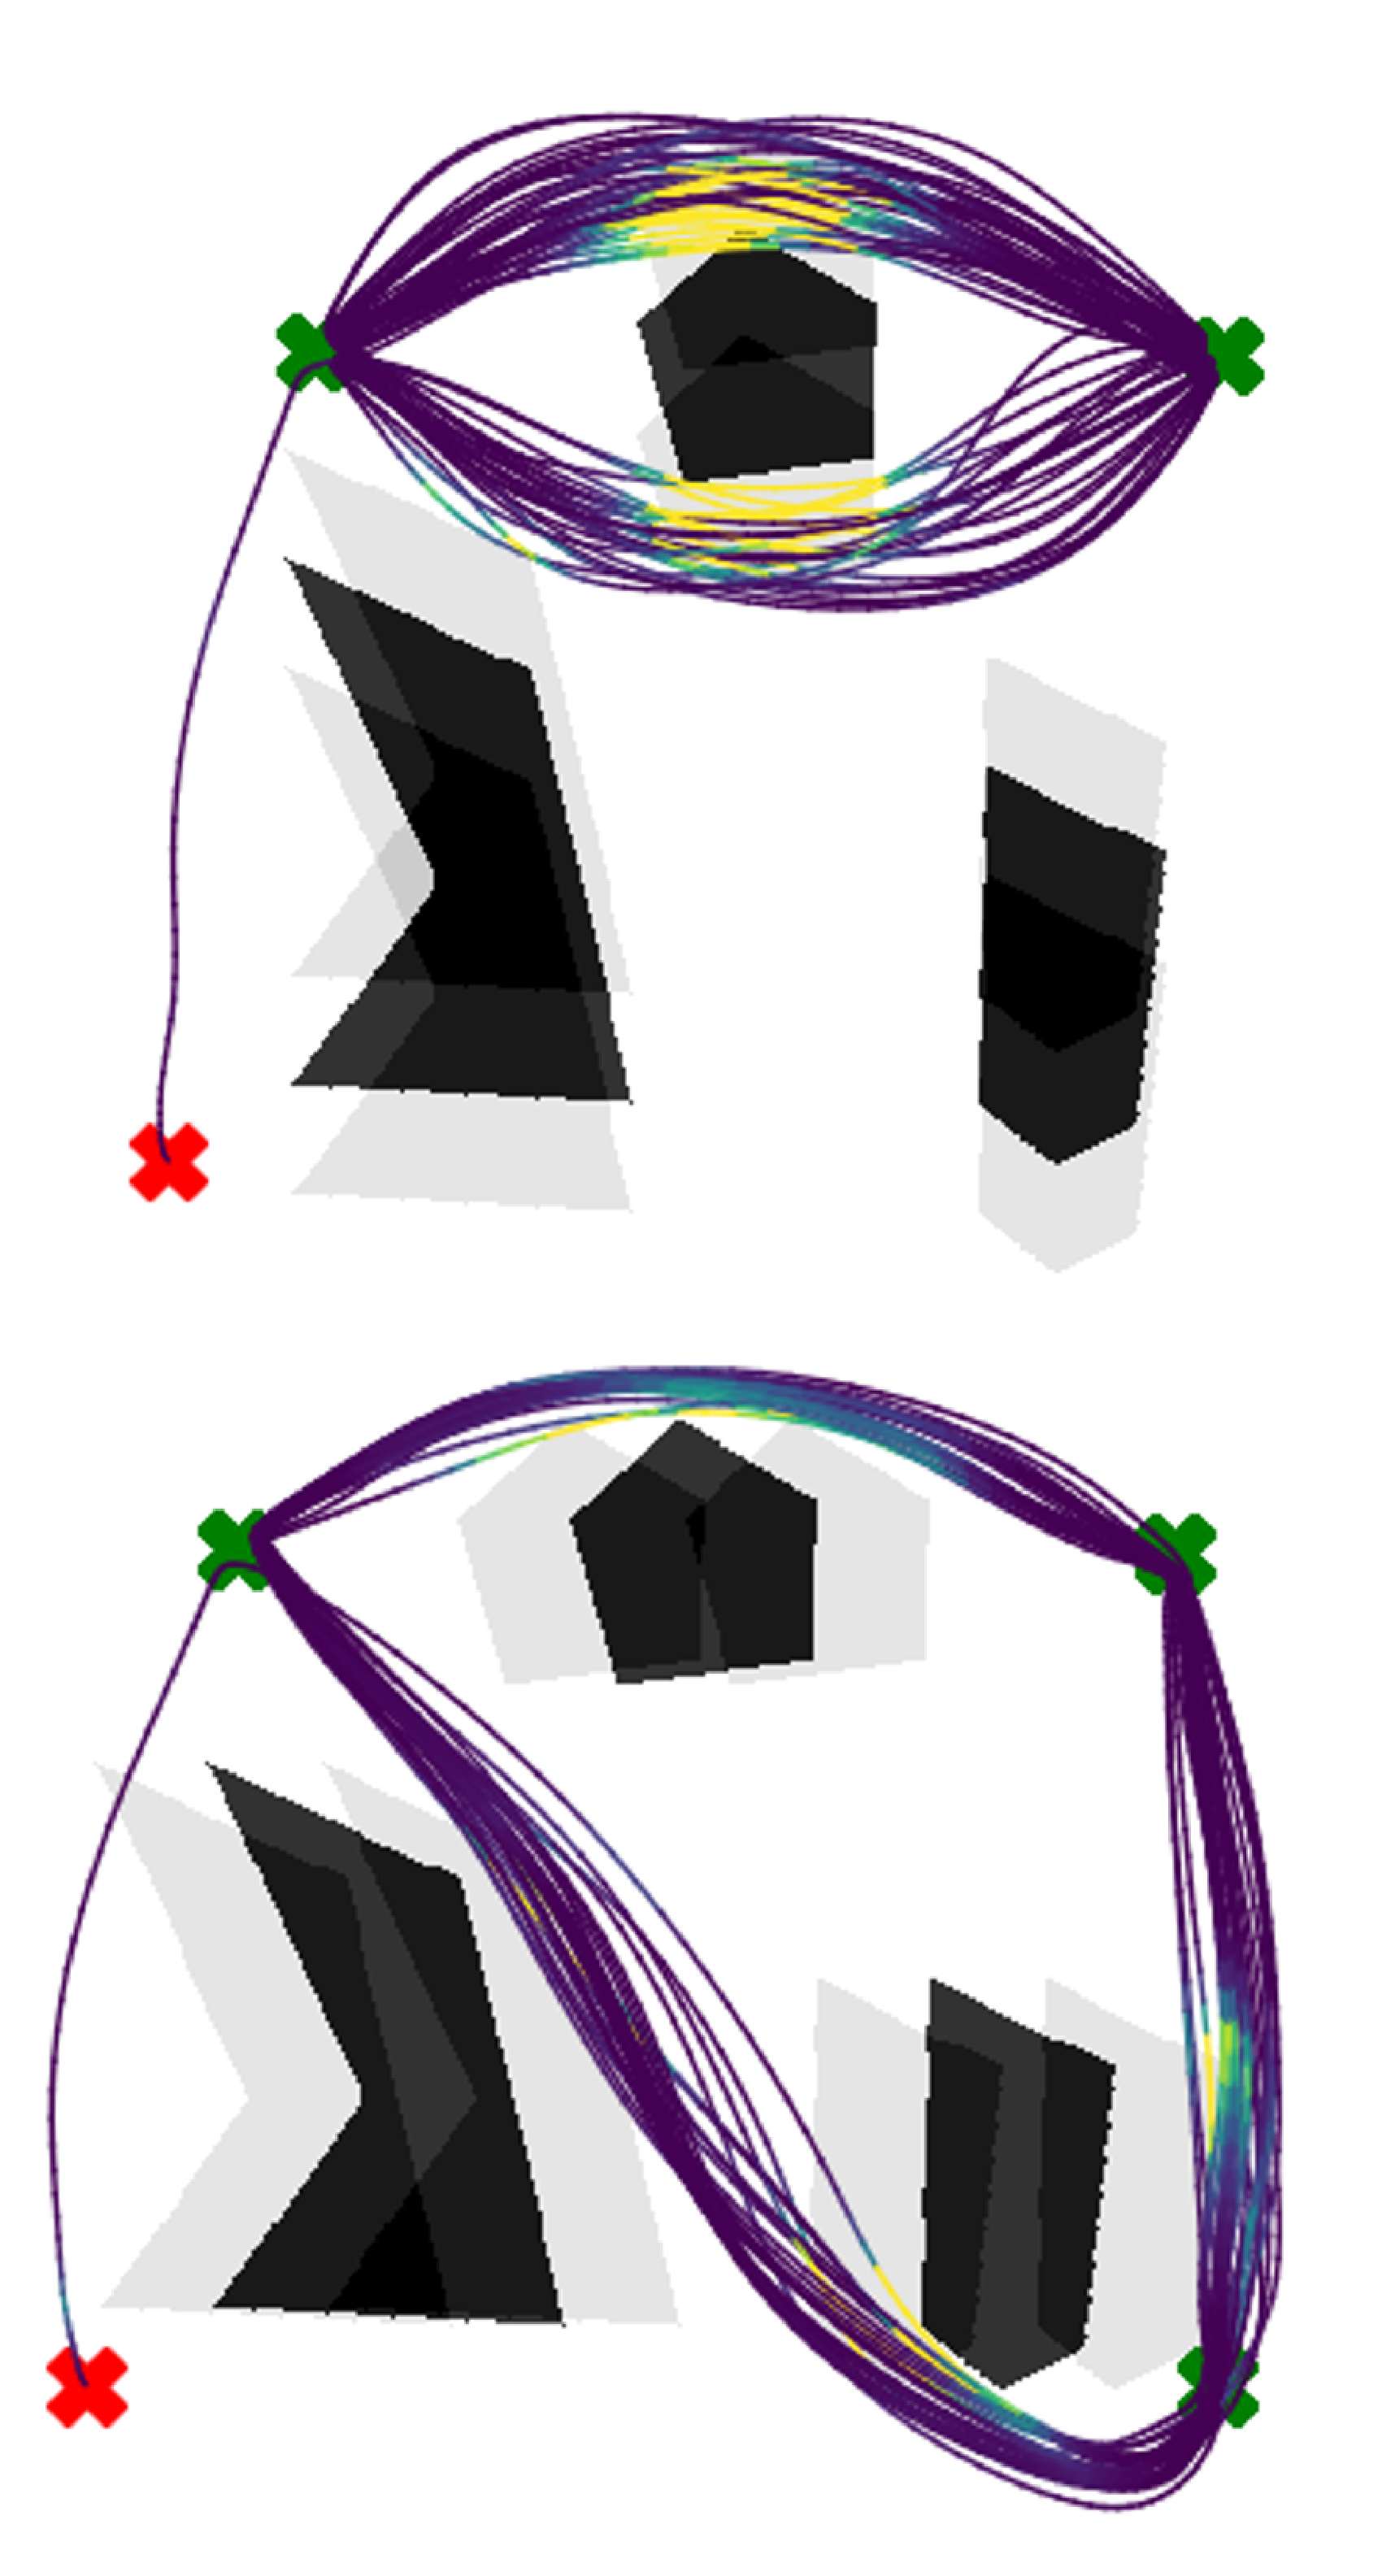
\includegraphics[width=\linewidth]{coll_c.eps}
		\caption{$(c)$}
	\end{subfigure}
	\hfill
	\begin{subfigure}[b]{0.11\textwidth}
		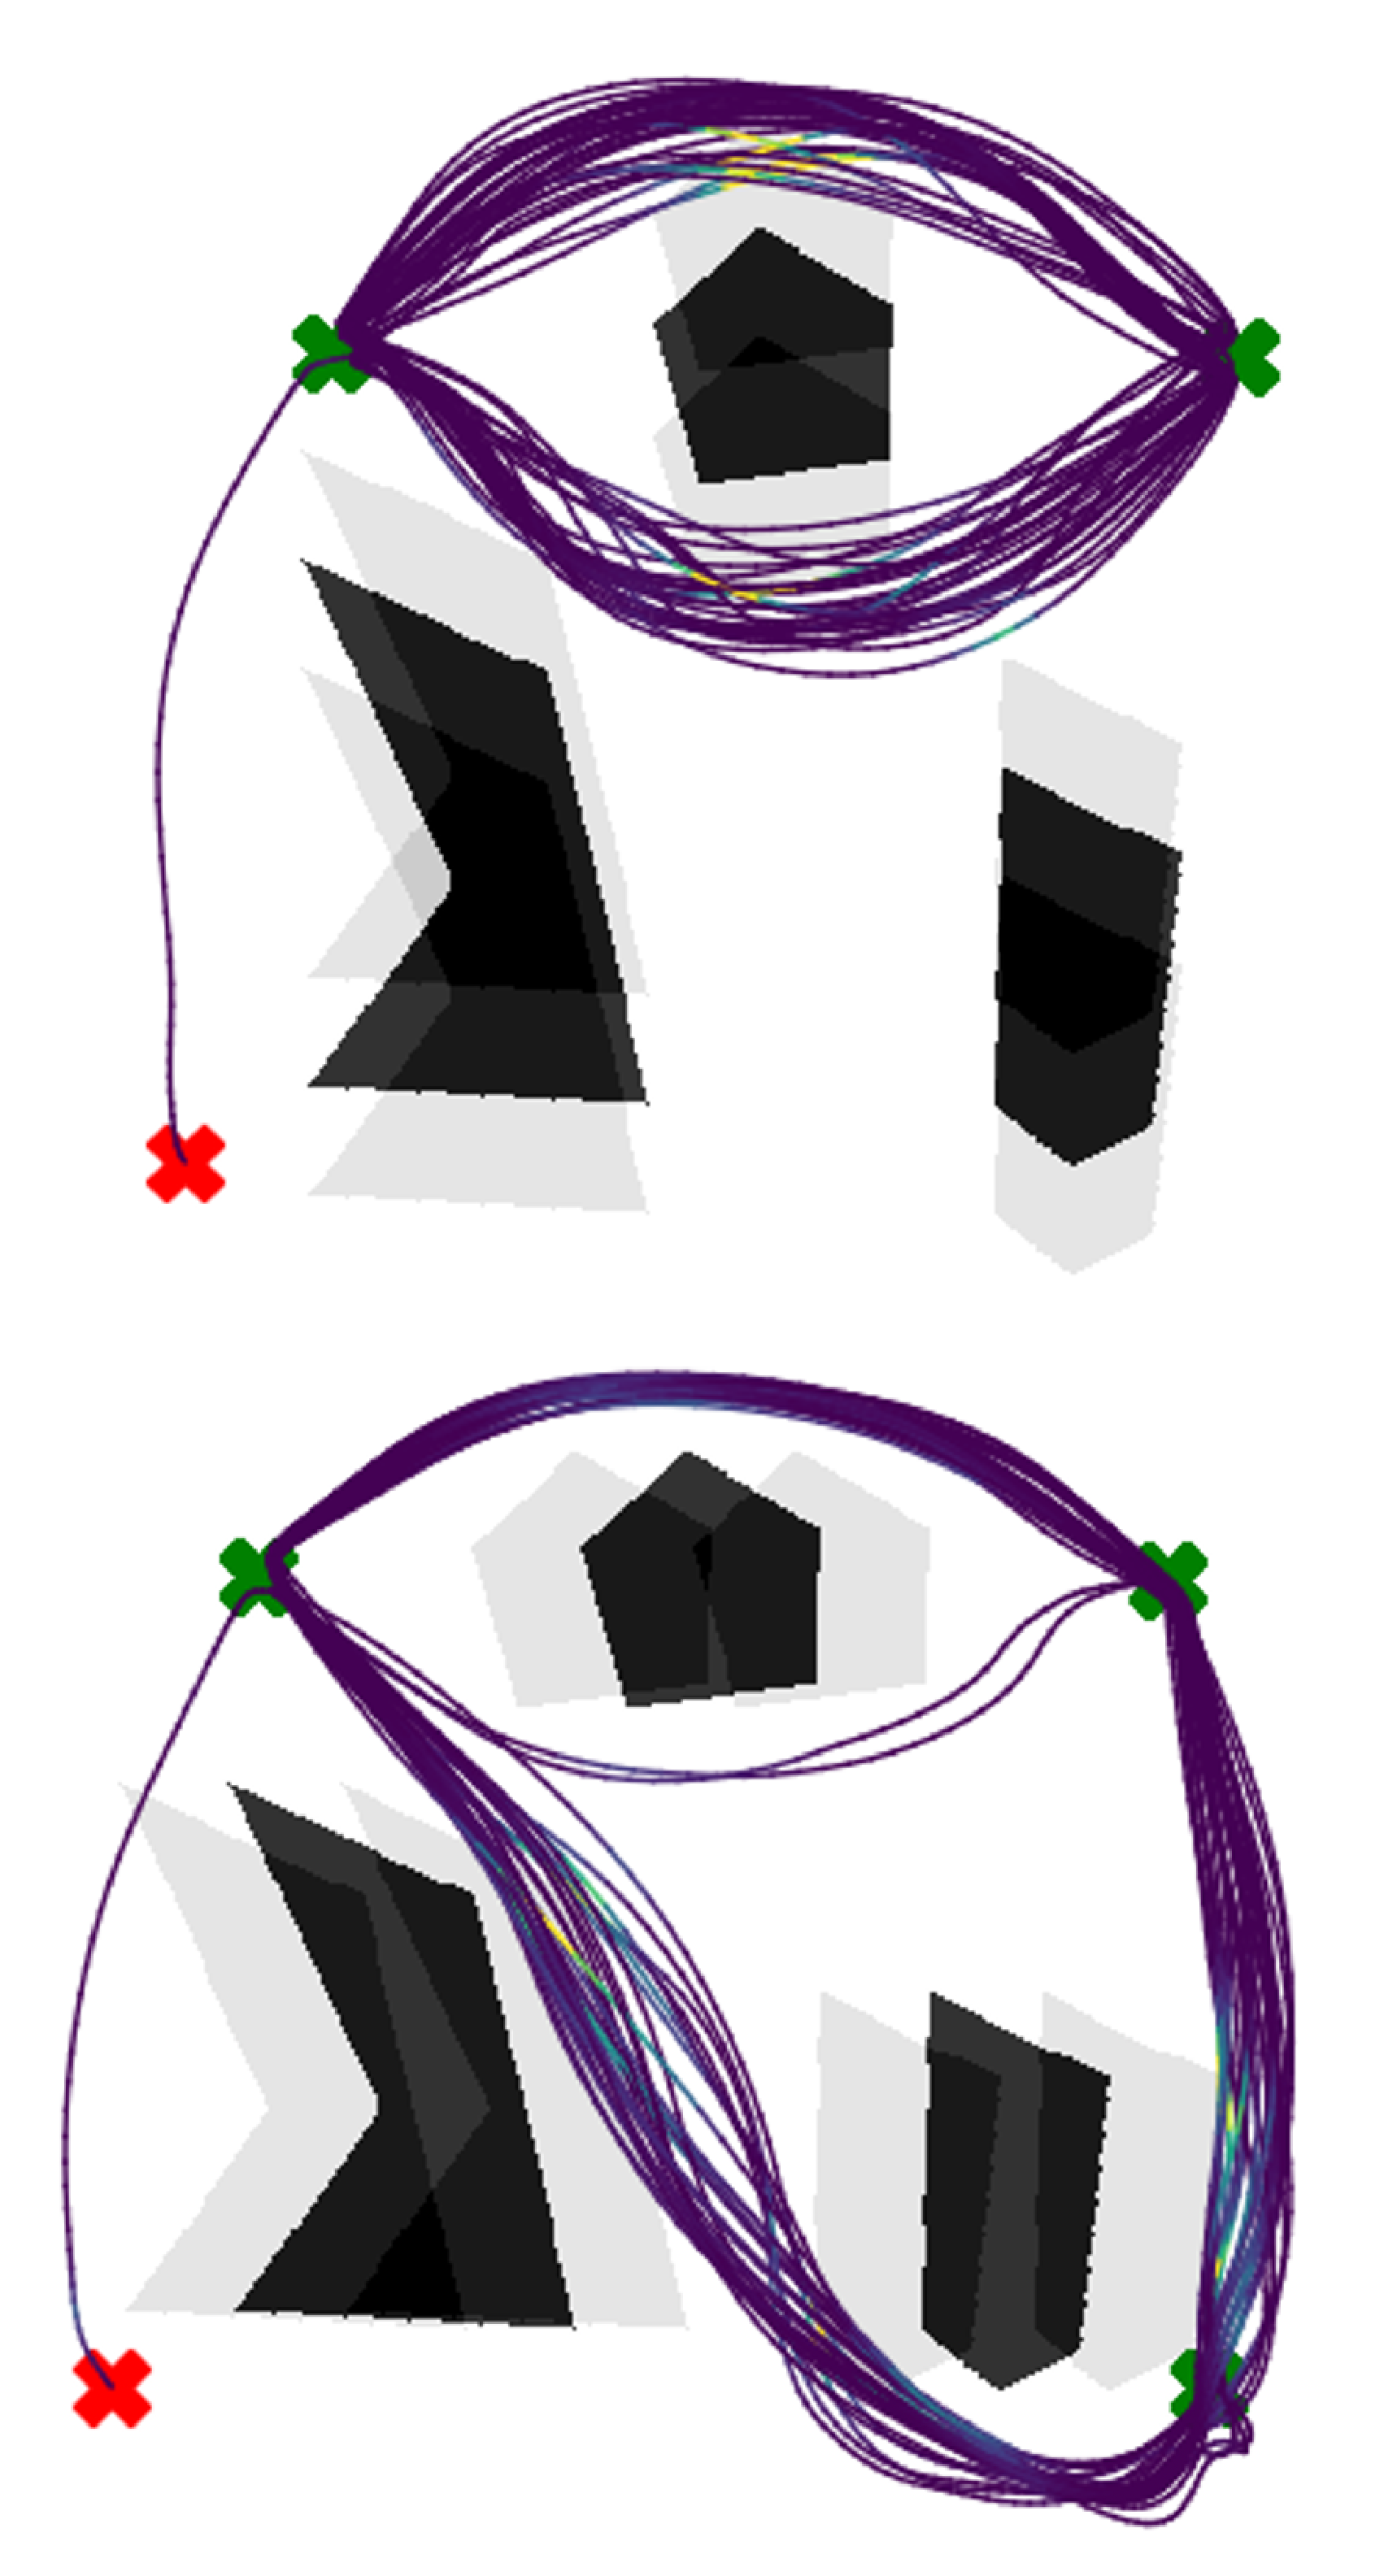
\includegraphics[width=\linewidth]{coll_d.eps}
		\caption{$(d)$}
	\end{subfigure}

	\caption{ .}
\end{figure}



------------- \\ 
Remark. 
Contributions to the Transactions, Journals, and Letters must be submitted electronically on IEEE's on-line manuscript submission and peer-review system, ScholarOne� Manuscripts (former Manuscript Central).

Before submitting, carefully read the TIE checklist above ``TIE checklist for new manuscript submissions'' and modify your manuscript accordingly. Once your paper completely satisfies the TIE rules, follow this procedure:

\begin{enumerate}[1)]
	\item Open ScholarOne� Manuscripts web \url{http://mc.manuscriptcentral.com/tie-ieee}. If you do not have an existing account, please create it. All IEEE journals require an Open Researcher and Contributor ID (ORCID) for all authors. ORCIDs enable accurate attribution and improved discoverability of an author's published work. The author will need a registered ORCID in order to submit a manuscript or review a proof in this journal.
	\item Go to your Author Center and click ``Submit First Draft of a New Manuscript''.
	\item Along with other information, you will be asked to select the subject from a pull-down list. There are various steps in the submission process; you must complete all steps for a complete submission. At the end of each step you must click ``Save and Continue''.
	\item Just uploading the paper is not sufficient. After the last step, you should see a confirmation that the submission is complete. You should also receive an e-mail confirmation.
	\item More detailed instructions can be found at \url{http://mchelp.manuscriptcentral.com/gethelpnow/training/author/}.
\end{enumerate}

Please notice that in your Author Center you may check the current status of your manuscript such as: In EIC office, Assigned to AE, AE invites reviewers, AE assigns reviewers, Under review, Awaiting AE decision, and Awaiting EIC decision. If you find that your manuscript is not moving in the process for a month or more please contact the Editor-in-Chief.

\subsection{TIE checklist for manuscript submissions}

Authors should consider the following points before submitting a new paper. Otherwise the submission will be automatically rejected.

\begin{enumerate}[1)]
	\item New manuscripts cannot exceed \textbf{8 pages} (3 for letters). Only a very limited overlength (1/2 page at most) is tolerated. Note that usually in the review process the reviewers tend to ask for more explanations, also note that the maximum allowed length is 8 pages on initial/first submission, including authors' bios and photos.
	\item In order to follow the \textbf{single-blind} review process, we ask that all the authors be identifiable within the manuscript (DO include authors' names, their biographies, affiliation, etc.). The articles in this journal are peer reviewed in accordance with the requirements set forth in the IEEE Publication Services and Products Board Operations Manual (https://pspb.ieee.org/images/files/files/opsmanual.pdf). Each published article was reviewed by a minimum of two independent reviewers using a single-blind peer review process, where the identities of the reviewers are not known to the authors, but the reviewers know the identities of the authors. Articles will be screened for plagiarism before acceptance.
	\item If a significant portion of your manuscript was already published at a conference you must use our \textbf{``Post Conference Papers'' template}. The manuscript must include the previous work in the references section. 
	\item TIE policy \textbf{doesn't consider surveys}, state of the art papers or project reports. Only Guest Editors of a special section (or submissions allowed by the Editorial Board) are invited to submit such kind of manuscript. Our typical papers propose new methods and demonstrate their effectiveness through experimental results in combination with simulation results.
	\item The only file which has to be submitted (uploaded) is the \textbf{manuscript in PDF format} (Word files are also possible but please be sure that the file was properly converted by the submission system). In order to make it portable you must embed the non-standard fonts or avoid them in the PDF file. This is not an easy process, but often all problems are solved when you are printing PDF file from Word and you will select in printer properties  ``Press Quality'' instead of ``Standard''.
	\item Manuscripts must be in IEEE \textbf{double column format} and follow all other IEEE guidelines described in this document, so the length of the paper and readability of figures can be evaluated.
	\item The file maximum size \textbf{cannot exceed 40MB} to make it accessible to our tools. Usually you will get that by adjusting the size of the figures. Note that ``EPS'' figures format is required only on the Final Stage.
	\item IEEE T IE is an application oriented engineering journal. It is therefore expected that all submissions will \textbf{contain experimental verification} of the novel theoretical concepts, given in the paper. Papers not containing experimental results should therefore not be submitted since they will be subject to an ``Immediate reject'' decision. An experimental rig, which must be used by the authors for verification, must contain hardware components other than a PC/laptop.	
	\item It is a mandatory requirement that the primary e-mail address of all authors is an \textbf{institutional e-mail}. This applies to all authors of each new and revised paper. Papers where this is not satisfied will not enter the review process.
	\item Your manuscript must be \textbf{within the scope of IEEE Trans. on Industrial Electronics}. If not, we will not be able to provide adequate review.
	\item \textbf{All cited papers must be referenced} within the text of the manuscript. Be sure that the manuscript is up to date. It is expected that a significant portion of references are to recently published papers.
	\item Your manuscript must have \textbf{abstract correctly written}. In the age of electronic publications it is not easy to be noticed (Industrial Electronics Society alone receives over 15,000 conference and journal papers per year). Authors have to do everything possible so the paper will be noticed and read. Therefore, very careful wording should be used in the title, abstract and index terms. Without those a great paper might never be found and read from IEEE Xplore.
	\item Your paper should describe very clearly your accomplishments so other people can understand what your \textbf{original contribution } is and use it. Notice that usually your technical accomplishments will be evaluated based on the number of citations but not based on the number of papers published.
	\item \textbf{Write clearly your manuscript}. Try to keep your manuscript on the proper level from one section to another. It should be easy to understand by well-qualified professionals, but at the same time please avoid describing well-known facts (use proper references instead). Often manuscripts receive negative reviews because reviewers are not able to understand the manuscript and this is authors' (not reviewers') fault. Notice, that if reviewers have difficulties, then other readers will face the same problem and there is no reason to publish the manuscript.
\end{enumerate}


\section{Submission of a Revised Manuscript for Review}

If an editor decides not to accept your manuscript, they may provide you with a decision that allows for reconsideration. If so, open ScholarOne� Manuscripts web \url{http://mc.manuscriptcentral.com/tie-ieee} and find the paper on your submission dashboard. The ``Actions'' column provides you with links to create a revision (for decision types of Minor Revision or Major Revision) or a resubmission (for decision type of Reject with Resubmit).

The checklist above ``TIE checklist for manuscript submissions'' also applies to the revised stage.

In the revision flow, the reviewers tend to ask for more explanations, also note that the maximum allowed length is 8 pages and exceptionally up to 10 pages may be authorized (paying an overlength fee). Note that the page count includes the authors' bios and photos

In the resubmission flow, please include a cover letter that mentions this paper number and describes the major changes to the manuscript. In particular, please summarize the new results that have been added. This should be accompanied by a point by point explanation of 1) how the previous comments from the reviewers were addressed and 2) how new results added to the paper make it stronger and increase the research contribution. The response to reviewers should be uploaded as a ``supplementary file,'' in addition to being uploaded as a cover letter so that all reviewers will have access to the file. Lastly, please make sure to highlight the changes in the paper (or at least use a different font color). If the changes are too much, highlight the major additions to the paper. Please do not submit a paper with track changes, as track changes make the paper difficult for reviewers to read.


\section{Submission of a Final Manuscript}

If an editor decides to accept your manuscript, you will receive via email an ``acceptance'' decision. In ScholarOne� Manuscripts, the status of your paper will be ``Awaiting Final Files'' and you will be able to submit the final manuscript.

The checklist above ``TIE checklist for manuscript submissions'' also applies to the final stage, with some exceptions:

\begin{enumerate}[1)]
	\item Author names list, footnote on the first page, optional acknowledgement section and authors' bios and photos must be included from the first submission. Letters to editor should not include authors' bios and photos.
	\item Please tailor your paper so its length does not exceed the 8 pages limit (up to 10 pages with fees) and the last page is not half empty. Note that the page count includes footnotes, acknowledgement, author photos and bios. If your paper after editing at IEEE HQ will run to a new page the editor may remove your photos and/or bios.
	\item Please notice that there are mandatory overlength charges of \$250 per page (\$200 for IES members), up to 10 pages.
	\item This submission must include the final list of references. Any later change will cause prolonged delays in the publishing process.
\end{enumerate}
	
Upon acceptance, you will receive an email with specific instructions regarding the submission of your final files.  To avoid any delays in publication, please be sure to follow these instructions. Final submissions should include source files of your accepted manuscript, high quality graphic files, and a formatted PDF file. If you have any questions regarding the final submission process, please contact the administrative contact for the journal.

\subsection{Final files:}

\begin{enumerate}[1)]
	\item A source file of your manuscript in either Microsoft Word or LaTeX. Save the document as TXT\_xx-TIE-xxxx.doc (Word file) or TXT\_xx-TIE-xxxx.tex (LaTeX project).
	\item  A publication-ready PDF of the manuscript which will appear as Early Access article on IEEE Xplore. The publication-ready PDF must match the source file. This PDF file must be made following all IEEE and TIE guide styles. When printing to PDF from Word in printer properties, select  ``Press Quality'' instead of ``Standard'' so the file meets IEEE Xplore requirements. Name this file as ALL\_xx-TIE-xxxx.pdf.
	\item If applicable, all supplemental material such as multimedia or graphical abstract.
	\item If the figures are not embedded into the text, then save all your figures in one or several documents. FIG1\_xx-TIE-xxxx.ext. Proper extensions are PS, EPS, TIFF, Microsoft Word, Microsoft PowerPoint, Microsoft Excel, or PDF.	If the author photos are not embedded in the text, and only for regular papers (4 to 8 pages, up to 10 with fees), then include color photos of each author with proper format (TIF, JPEG, EPS, PDF, DOC, or PPT) and proper resolution (300 dpi). Name each photo as AUTHOR\_NAME.ext. Letters (up to 3 printed pages) must not have biographies or photos of authors.
\end{enumerate}

Pack everything to one zip file xx-TIE-xxxx.zip and upload into ScholarOne� Manuscripts.

Once authors upload final files in ScholarOne� Manuscripts, they will be automatically redirected to a new IEEE page where they can sign the eCF.

As a summary, the zip file should include the following files:

\begin{enumerate}[1)]
	\item TXT\_xx-TIE-xxxx.doc or TXT\_xx-TIE-xxxx.tex - \textbf{Source file} of your manuscript.	
	\item ALL\_xx-TIE-xxxx.pdf -  A \textbf{publication-ready PDF} of the manuscript which will appear as Early Access article on IEEE Xplore. The publication-ready PDF must match the source file.
	\item If applicable, all \textbf{supplemental material} such as multimedia or graphical abstract.
	\item \textbf{Figures} [FIG1\_xx-TIE-xxxx.ext] in the acceptable format (if they are not embedded into the text). \textbf{Author photos} [AUTHOR\_NAME.ext], only for Regular Papers (if they are not embedded into the text).
	
\end{enumerate}

The zip file xx-TIE-xxxx.zip should be uploaded into ScholarOne� Manuscripts.

You are strongly encouraged to use TeX, LaTeX or Troff programs for the most accurate and efficient transfer of your manuscript, especially for those containing extensive mathematics.


\section{Guidelines for Manuscript Preparation}
A general IEEE style guide is available at \url{https://ieeeauthorcenter.ieee.org/}.

\subsection{Abbreviations and Acronyms}
Define abbreviations and acronyms the first time they are used in the text, even after they have already been defined in the abstract. Abbreviations such as IEEE, SI, ac, and dc do not have to be defined. Abbreviations that incorporate periods should not have spaces: write ``C.N.R.S.,'' not ``C. N. R. S.'' Do not use abbreviations in the title unless they are unavoidable (for example, ``IEEE'' in the title of this article).	

\subsection{Other Recommendations}
Use one space after periods and colons. Hyphenate complex modifiers: ``zero-field-cooled magnetization.'' Avoid dangling participles, such as, ``Using (1), the potential was calculated.'' [It is not clear who or what used (1).] Write instead, ``The potential was calculated by using (1),'' or ``Using (1), we calculated the potential.''

Use a zero before decimal points: ``0.25,'' not ``.25.'' Use ``cm3,'' not ``cc.'' Indicate sample dimensions as ``0.1 cm x 0.2 cm,'' not ``0.1 x 0.2 cm2.'' The abbreviation for ``seconds'' is ``s,'' not ``sec.'' Use ``Wb/m2'' or ``webers per square meter,'' not ``webers/m2.'' When expressing a range of values, write ``7 to 9'' or ``7-9,'' not ``7~9.''.

\section{Maths}

If you are using Word, use either the Microsoft Equation Editor or the MathType add-on (http://www.mathtype.com) for equations in your paper (Insert | Object | Create New | Microsoft Equation or MathType Equation). ``Float over text'' should not be selected.

\subsection{Equations}
Number equations consecutively with equation numbers in parentheses flush with the right margin, as in (1). First use the equation editor to create the equation. Then select the ``Equation'' markup style. Press the tab key and write the equation number in parentheses. To make your equations more compact, you may use the solidus ( / ), the exp function, or appropriate exponents. Use parentheses to avoid ambiguities in denominators. Punctuate equations when they are part of a sentence, as in	


\begin{align}
\nonumber\mathbf \int_{0}^{{r}_2} & F(r,\varphi) dr \ d\varphi = [\sigma{r}_2 / (2{\mu}_0)]
\\
& \int_{0}^{\infty} exp(-\lambda|{z}_j - {z}_i|){\lambda}^{-1} {J}_1 (\lambda {r}_2) {J}_0 (\lambda {r}_i) d \lambda .
\end{align}


Be sure that the symbols in your equation have been defined before the equation appears or immediately following. Italicize symbols (T might refer to temperature, but T is the unit tesla). Refer to ``(1),'' not ``Eq. (1)'' or ``equation (1),'' except at the beginning of a sentence: ``Equation (1) is ...'' .
		
\section{Units}

Use either SI (MKS) or CGS as primary units. (SI units are strongly encouraged.) English units may be used as secondary units (in parentheses). This applies to papers in data storage. For example, write ``15 Gb/cm2 (100 Gb/in2).'' An exception is when English units are used as identifiers in trade, such as ``3�-in disk drive.'' Avoid combining SI and CGS units, such as current in amperes and magnetic field in oersteds. This often leads to confusion because equations do not balance dimensionally. If you must use mixed units, clearly state the units for each quantity in an equation.


\begin{figure}[!t]\centering
	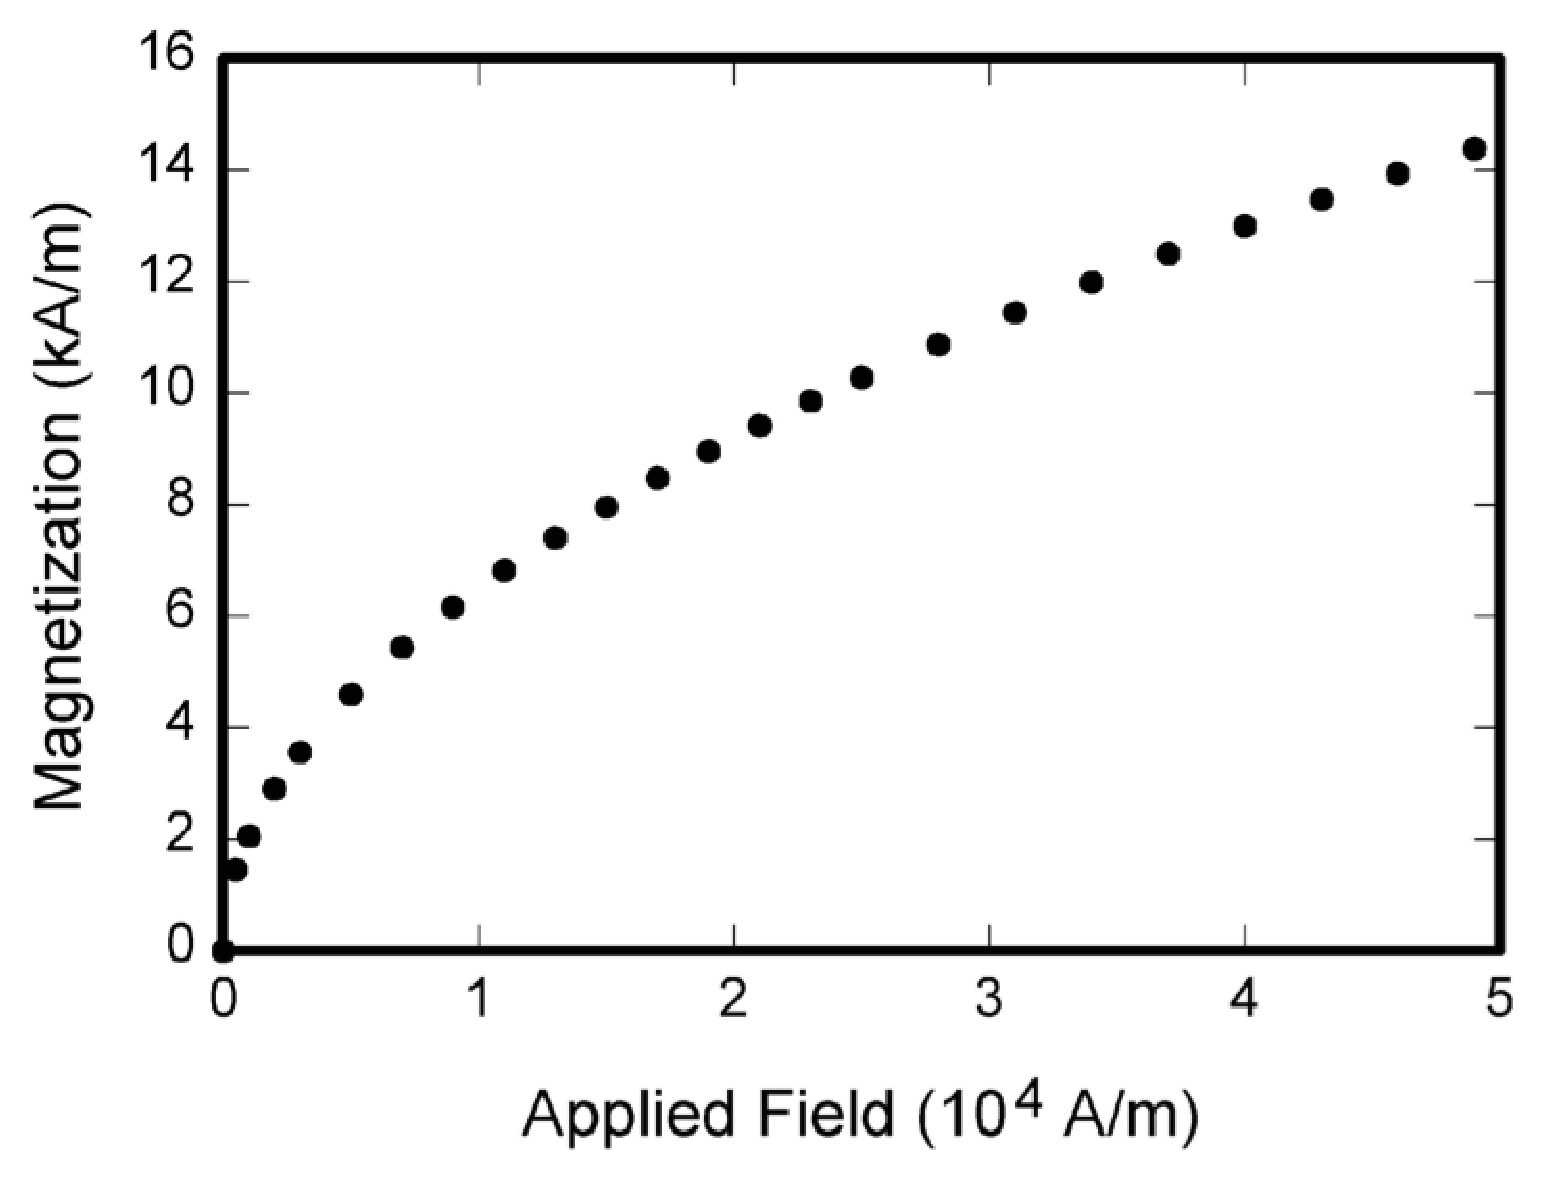
\includegraphics[width=8.5cm]{FIG1.eps}
	\caption{Magnetization as a function of applied field. Note that ``Fig.'' is abbreviated. There is a period after the figure number, followed by two spaces. It is good practice to explain the significance of the figure in the caption.}\label{FIG_1}
\end{figure}



The SI unit for magnetic field strength H is A/m. However, if you wish to use units of T, either refer to magnetic flux density B or magnetic field strength symbolized as \SI{}{\micro0H}. Use the center dot to separate compound units, e.g., ``A�m2.''

\section{Guidelines for Graphics Preparation and Submission}

\subsection{Types of Graphics}
The following list outlines the different types of graphics published in IEEE journals. They are categorized based on their construction, and use of color / shades of gray.

Such figures may include photographs, illustrations, multicolor graphs, and flowcharts.

Figures that are composed of only black lines and shapes. These figures should have no shades or half-tones of gray. Only black and white.

Head and shoulders shots of authors which appear at the end of our papers.  Data charts which are typically black and white, but sometimes include color.

\subsection{Multipart figures}

Figures compiled of more than one sub-figure presented side-by-side, or stacked. If a multipart figure is made up of multiple figure types (one part is lineart, and another is grayscale or color) the figure should meet the stricter guidelines.


\begin{table}[!t]
	\renewcommand{\arraystretch}{1.3}
	\caption{Units for Magnetic Properties}
	\centering
	\label{table_1}
	%\centering
	\resizebox{\columnwidth}{!}{
		\begin{tabular}{l l l}
			\hline\hline \\[-3mm]
			\multicolumn{1}{c}{Symbol} & \multicolumn{1}{c}{Quantity} & \multicolumn{1}{c}{\pbox{20cm}{Conversion from Gaussian and \\ \hphantom{spaces} CGS EMU to $ SI^{a} $ }}  \\[1.6ex] \hline
			$ \Phi $  & magnetic flux & $ 1Mx \rightarrow 10^8 Wb = 10^8 V \cdot s $ \\
			\pbox{20cm}{$ \emph{B} $ \\\hphantom{1}} & \pbox{20cm}{magnetic flux density, \\ \hphantom{1} magnetic induction} &  \pbox{20cm}{$ 1G \rightarrow 10^4 T = 10^4 Wb/m^2 $ \\ \hphantom{1}} \\ 
			$ \emph{H} $ & magnetic field strength & $ 1Oe \rightarrow 10^3/(4\pi)A/m $ \\
			\pbox{20cm}{$ \emph{m} $ \\ \hphantom{1}} & \pbox{20cm}{magnetic moment \\ \hphantom{1}} & \pbox{20cm}{$ 1 erg/G = 1 emu $ \\ \hphantom{1} $ \rightarrow 10^3 A \cdot m^2 = 10^3 J/T $ } \\ 
			\pbox{20cm}{$ \emph{M} $ \\ \hphantom{1}} & \pbox{20cm}{magnetization \\ \hphantom{1}} & \pbox{20cm}{$ 1 erg/(G \cdot cm^3) = 1 emu/cm^3 $ \\ \hphantom{1} $ \rightarrow 10^3 A/m $ } \\ 
			$ 4\pi\emph{M} $ & magnetization & $ 1G \rightarrow 10^3/(4\pi)A/m $ \\
			$ \sigma $ & specific magnetization & $ 1 erg/(G \cdot g) = 1 emu/g \rightarrow 1 A \cdot m^2/kg $ \\
			\pbox{20cm}{$ \emph{j} $ \\ \hphantom{1}} & \pbox{20cm}{magnetic dipole \\ \hphantom{1} moment } & \pbox{20cm}{$ 1 erg/G = 1 emu $ \\ \hphantom{1} $ \rightarrow 4\pi \times 10^{10} Wb \cdot m $ } \\ [1.4ex]
			\pbox{20cm}{$ \emph{J} $ \\ \hphantom{1}} & \pbox{20cm}{magnetic polarization \\ \hphantom{1}} & \pbox{20cm}{$ 1 erg/(G \cdot cm^3) = 1 emu/cm^3 $ \\ \hphantom{1} $ \rightarrow 4\pi \times 10^{4} T $ } \\ 
			$ \chi \ \kappa $ & susceptibility & $ 1 \rightarrow 4\pi $ \\ 
			$ \chi  $ & mass susceptibility & $ 1 cm^3/g \rightarrow 4\pi \times 10^{3} m^3/kg $ \\ 
			\pbox{20cm}{$ \mu $ \\ \hphantom{1}} & \pbox{20cm}{permeability \\ \hphantom{1}} & \pbox{20cm}{$ 1 \rightarrow 4\pi \times 10^{7} H/m $ \\ \hphantom{1} $ =4\pi \times 10^{7} Wb/(A \cdot m) $ } \\ 
			$ \mu_r $ & relative permeability & $ \mu \rightarrow \mu_r $ \\ 
			$ \omega, \emph{W} $ & energy density & $ 1 erg/cm^3 \rightarrow 10^1 J/m^3 $ \\ 
			$ \emph{N}, \emph{D} $ & demagnetizing factor & $ 1 \rightarrow 1/(4\pi) $ \\ [1.4ex]
			\hline\hline
		\end{tabular}
	}
\end{table}

\subsection{File Formats For Graphics}

Format and save your graphics using a suitable graphics processing program that will allow you to create the images as PostScript (PS), Encapsulated PostScript (.EPS), Tagged Image File Format (.TIFF), Portable Document Format (.PDF), or Portable Network Graphics (.PNG) sizes them, and adjusts the resolution settings. If you created your source files in one of the following programs you will be able to submit the graphics without converting to a PS, EPS, TIFF, PDF, or PNG file: Microsoft Word, Microsoft PowerPoint, or Microsoft Excel. Though it is not required, it is recommended that these files be saved in PDF format rather than DOC, XLS, or PPT. Doing so will protect your figures from common font and arrow stroke issues that occur when working on the files across multiple platforms. When submitting your final paper, your graphics should all be submitted individually in one of these formats along with the manuscript.


\subsection{Sizing of Graphics}

Most charts, graphs, and tables are one column wide (3.5 inches / 88 millimeters / 21 picas) or page wide (7.16 inches / 181 millimeters / 43 picas). The maximum depth a graphic can be is 8.5 inches (216 millimeters / 54 picas). When choosing the depth of a graphic, please allow space for a caption. Figures can be sized between column and page widths if the author chooses, however it is recommended that figures are not sized less than column width unless when necessary.

There is currently one publication with column measurements that don't coincide with those listed above. PROCEEDINGS OF THE IEEE has a column measurement of 3.25 inches (82.5 millimeters / 19.5 picas).

The final printed size of author photographs is exactly
1 inch wide by 1.25 inches tall (25.4 millimeters x 31.75 millimeters / 6 picas x 7.5 picas). Author photos printed in editorials measure 1.59 inches wide by 2 inches tall (40 millimeters  x 50 millimeters  / 9.5 picas x 12 picas).


\subsection{Resolution}

The proper resolution of your figures will depend on the type of figure it is as defined in the ``Types of Figures'' section. Author photographs, color, and grayscale figures should be at least 300dpi. Lineart, including tables should be a minimum of 600dpi.


\subsection{Vector Art}

While IEEE does accept, and even recommends that authors submit artwork in vector format, it is our policy is to rasterize all figures for publication. This is done in order to preserve the figures' integrity across multiple computer platforms.


\subsection{Color Space}

The term color space refers to the entire sum of colors that can be represented within the said medium. For our purposes, the three main color spaces are Grayscale, RGB (red/green/blue) and CMYK (cyan/magenta/yellow/black). RGB is generally used with on-screen graphics, whereas CMYK is used for printing purposes.

All color figures should be generated in RGB or CMYK color space. Grayscale images should be submitted in Grayscale color space. Line art may be provided in grayscale OR bitmap colorspace. Note that ``bitmap colorspace'' and ``bitmap file format'' are not the same thing. When bitmap color space is selected, .TIF/.TIFF is the recommended file format.


\subsection{Accepted Fonts Within Figures}

When preparing your graphics IEEE suggests that you use of one of the following Open Type fonts: Times New Roman, Helvetica, Arial, Cambria, and Symbol. If you are supplying EPS, PS, or PDF files all fonts must be embedded. Some fonts may only be native to your operating system; without the fonts embedded, parts of the graphic may be distorted or missing.

A safe option when finalizing your figures is to strip out the fonts before you save the files, creating ``outline'' type. This converts fonts to artwork what will appear uniformly on any screen.


\subsection{Using Labels Within Figures}

\begin{enumerate}
	\item Figure Axis labels\\
	Figure axis labels are often a source of confusion. Use words rather than symbols. As an example, write the label ``Magnetization,'' or ``Magnetization M,'' not just ``M.'' Put units in parentheses. Do not label axes only with units. As in \mbox{Fig. \ref{FIG_1}}, for example, write ``Magnetization (A/m)'' or ``Magnetization (A m1),'' not just ``A/m.'' Do not label axes with a ratio of quantities and units. For example, write ``Temperature (K),'' not ``Temperature/K.''. Multipliers can be especially confusing. Write ``Magnetization (kA/m)'' or ``Magnetization (103 A/m).'' Do not write ``Magnetization (A/m) x 1000'' because the reader would not know whether the top axis label in \mbox{Fig. \ref{FIG_1}} meant 16000 A/m or 0.016 A/m. Figure labels should be legible, approximately 8 to 10 point type.	
	\item Subfigure Labels in Multipart Figures and Tables\\
	Multipart figures should be combined and labeled before final submission. Labels should appear centered below each subfigure in 8 point Times New Roman font in the format of (a) (b) (c). 	
\end{enumerate}

\subsection{Referencing a Figure or Table Within Your Paper}
When referencing your figures and tables within your paper, use the abbreviation ``Fig.'' even at the beginning of a sentence. Do not abbreviate ``Table.'' Tables should be numbered with Roman Numerals.

\subsection{Checking Your Figures: The IEEE Graphics Checker}
The IEEE Graphics Checker Tool enables authors to pre-screen their graphics for compliance with IEEE Transactions and Journals standards before submission. The online tool, located at \url{http://graphicsqc.ieee.org/}, allows authors to upload their graphics in order to check that each file is the correct file format, resolution, size and colorspace; that no fonts are missing or corrupt; that figures are not compiled in layers or have transparency, and that they are named according to the IEEE Transactions and Journals naming convention. At the end of this automated process, authors are provided with a detailed report on each graphic within the web applet, as well as by email.

For more information on using the Graphics Checker Tool or any other graphics related topic, contact the IEEE Graphics Help Desk by e-mail at graphics@ieee.org.

\subsection{Submitting Your Graphics}
Because IEEE will do the final formatting of your paper, you do not need to position figures and tables at the top and bottom of each column. In fact, all figures, figure captions, and tables can be placed at the end of your paper. In addition to, or even in lieu of submitting figures within your final manuscript, figures should be submitted individually, separate from the manuscript in one of the file formats listed above in section VI-J. Place figure captions below the figures; place table titles above the tables. Please do not include captions as part of the figures, or put them in ``text boxes'' linked to the figures. Also, do not place borders around the outside of your figures.

\subsection{Color Processing / Printing in IEEE Journals}
All IEEE Transactions, Journals, and Letters allow an author to publish color figures on IEEE Xplore� at no charge, and automatically convert them to grayscale for print versions. In most journals, figures and tables may alternatively be printed in color if an author chooses to do so. Please note that this service comes at an extra expense to the author. If you intend to have print color graphics, include a note with your final paper indicating which figures or tables you would like to be handled that way, and stating that you are willing to pay the additional fee.


\section{Conclusion}

A conclusion section is not required. Although a conclusion may review the main points of the paper, do not replicate the abstract as the conclusion. A conclusion might elaborate on the importance of the work or suggest applications and extensions.


\section*{Appendix}

Appendixes, if needed, appear before the acknowledgment.

\section*{Acknowledgment}

The preferred spelling of the word ``acknowledgment'' in American English is without an ``e'' after the ``g.'' Use the singular heading even if you have many acknowledgments. Avoid expressions such as ``One of us (S.B.A.) would like to thank ... .'' Instead, write ``F. A. Author thanks ... .'' In most cases, sponsor and financial support acknowledgments are placed in the unnumbered footnote on the first page, not here.

\section*{References and Footnotes}

\subsection{References}
References need to be cited in text. Put the number on the line, in square brackets inside the punctuation.  Multiple references are each numbered with separate brackets. When citing a section in a book, please give the relevant page numbers. In text, refer simply to the reference number. Do not use ``Ref.'' or ``reference'' except at the beginning of a sentence: ``Reference [\#] shows ... .'' Please do not use automatic endnotes in Word, rather, type the reference list at the end of the paper using the ``References'' style.

Reference numbers are set flush left and form a column of their own, hanging out beyond the body of the reference. The reference numbers are on the line, enclosed in square brackets. In all references, the given name of the author or editor is abbreviated to the initial only and precedes the last name. Use them all; use et al. exceptionally if more than 6 author names were listed. Use commas around Jr., Sr., and III in names. Abbreviate conference titles \cite{inproceedings1}.  When citing journals \cite{article1, article2, article3, article4, article5, article6, article7, article8, article9, article10}, provide the issue number, page range, volume number, DOI, year, and/or month if available. When referencing a patent \cite{patent1}, provide the day and the month of issue, or application. References may not include all information; please obtain and include relevant information. Do not combine references. There must be only one reference with each number. If there is a URL included with the print reference, it can be included at the end of the reference \cite{onlinebook1}.

Authors are encouraged to include the DOI number for each reference. It's the most important part of the reference. The DOI is like a digital fingerprint and it's used to identify the article without mistakes.

Other than books \cite{inbook1, book1, book2, book3}, capitalize only the first word in a paper title, except for proper nouns and element symbols. For papers published in translation journals, please give the English citation first, followed by the original foreign-language citation See the end of this document for formats and examples of common references. For a complete discussion of references and their formats, see ``The IEEE Style Manual,'' available as a PDF link off the Author Digital Toolbox main page.

\subsection{Footnotes}
Number footnotes separately in superscripts (Insert | Footnote).\footnote{It is recommended that footnotes be avoided (except for the unnumbered footnote with the receipt date on the first page). Instead, try to integrate the footnote information into the text.}  Place the actual footnote at the bottom of the column in which it is cited; do not put footnotes in the reference list (endnotes). Use letters for table footnotes  (see \mbox{Table \ref{table_1}}).


\section{Editorial Policy}

Do not submit a reworked version of a paper you have submitted or published elsewhere. Do not publish ``preliminary'' data or results. The submitting author is responsible for obtaining agreement of all coauthors and any consent required from sponsors before submitting a paper.

The IEEE Transactions and Journals Department does not publish conference records or proceedings. The department  does publish papers related to conferences that have been recommended for publication on the basis of peer review. As a matter of convenience and service to the technical community, these topical papers are typically collected and published in one special issue of most transactions publications.

At least two reviews are required for every paper submitted. Indecipherable English is a valid reason for rejection. There is a service available that will help you improve your English for a fee, and the link to that service can be found at \url{https://ieeeauthorcenter.ieee.org/}.

Authors of rejected papers may revise and resubmit them as regular papers, whereupon they will be reviewed by two new referees.

\section{Publication Principles}

The two types of contents of that are published are; 1) peer-reviewed and 2) archival. The Transactions and Journals Department publishes scholarly articles of archival value as well as tutorial expositions and critical reviews of classical subjects and topics of current interest.
Authors should consider the following points:

\begin{enumerate}[1)]
\item Technical papers submitted for publication must advance the state of knowledge and must cite relevant prior work.
\item The length of a submitted paper should be commensurate with the importance, or appropriate to the complexity, of the work. For example, an obvious extension of previously published work might not be appropriate for publication or might be adequately treated in just a few pages.
\item Authors must convince both peer reviewers and the editors of the scientific and technical merit of a paper; the standards of proof are higher when extraordinary or unexpected results are reported.
\item Because replication is required for scientific progress, papers submitted for publication must provide sufficient information to allow readers to perform similar experiments or calculations and use the reported results. Although not everything need be disclosed, a paper must contain new, useable, and fully described information. For example, a specimen's chemical composition need not be reported if the main purpose of a paper is to introduce a new measurement technique. Authors should expect to be challenged by reviewers if the results are not supported by adequate data and critical details.
\item Papers that describe ongoing work or announce the latest technical achievement, which are suitable for presentation at a professional conference, may not be appropriate for publication.
\end{enumerate}



% References

\bibliographystyle{Bibliography/IEEEtranTIE}
\bibliography{Bibliography/IEEEabrv,Bibliography/BIB_xx-TIE-xxxx}\ %IEEEabrv instead of IEEEfull

	
%\vspace{-1cm}
\begin{IEEEbiography}[{
\includegraphics[width=1in,height=1.25in,clip,keepaspectratio]{photo-men.eps}}]
{First A. Author1} and the other authors may include biographies at the end of regular papers. The first paragraph may contain a place and/or date of birth (list place, then date). Next, the author's educational background is listed. The degrees should be listed with type of degree in what field, which institution, city, state or country, and year degree was earned. The author's major field of study should be lower-cased.

The second paragraph uses the pronoun of the person (he or she) and not the author's last name. It lists military and work experience, including summer and fellowship jobs. Job titles are capitalized. The current job must have a location; previous positions may be listed without one. Information concerning previous publications may be included.

The third paragraph begins with the author's title and last name (e.g., Dr. Smith, Prof. Jones, Mr. Kajor, Ms. Hunter). List any memberships in professional societies other than the IEEE. Finally, list any awards and work for IEEE committees and publications. If a photograph is provided, the biography will be indented around it. The photograph is placed at the top left of the biography. Personal hobbies will be deleted from the biography.
\end{IEEEbiography}

%\vspace{-1cm}
\begin{IEEEbiography}[{
\includegraphics[width=1in,height=1.25in,clip,keepaspectratio]{photo-men.eps}}]
{Second B. Author2} (M'12) was born in City, Country. He received the M. degree in electrical engineering from University of City, Country in 2012.

The second paragraph uses the pronoun of the person (he or she) and not the author's last name. It lists military and work experience, including similar information to the previous author, including military, work experience, and other jobs. Job titles are capitalized. The current job must have a location; previous positions may be listed without one. Information concerning previous publications may be included.

The third paragraph begins with the author's title and last name (e.g., Dr. Smith, Prof. Jones, Mr. Kajor, Ms. Hunter), including similar information to the previous author, including the list of any awards and work for IEEE committees and publications. The photograph is placed at the top left of the biography. Personal hobbies will be deleted from the 
biography.
\end{IEEEbiography}

%\vspace{-2cm}
\begin{IEEEbiography}[{
\includegraphics[width=1in,height=1.25in,clip,keepaspectratio]{photo-men.eps}}]
{Third C. Author3} (M'99-SM'04-F'09) was born in City, Country. He received the M. and SM. and F. degrees in electrical engineering from University of City, Country in 1999, 2004 and 2009 respectively.

The second paragraph uses the pronoun of the person (he or she) and not the author's last name. It lists military and work experience, including similar information to the previous author, including military, work experience, and other jobs.

The third paragraph begins with the author's title and last name (e.g., Dr. Smith, Prof. Jones, Mr. Kajor, Ms. Hunter), including similar information to the previous author, including the list of any awards and work for IEEE committees and publications. The photograph is placed at the top left of the biography. Personal hobbies will be deleted from the biography.
%\\ \\ 
\end{IEEEbiography}


\end{document}
